% !Mode:: "TeX:UTF-8" 

\BiChapter{克隆代码创建一致性维护需求预测方法}
{Predicting Clone Creating Consistency-Requirement at Copy-and-Paste Time}

\BiSection{引言}
{Introduction}

在软件开发过程中,程序开发人员通过复制和粘贴操作复用软件中既有的代码,从而向系统中引入新的克隆代码。新产生的克隆代码在随着软件系统的演化过程中,可能会发生一致性变化而导致软件的额外维护代价。遗忘该一致性变化还会引入与之相关的克隆一致性违背缺陷,从而将进一步增大系统的维护代价。因此,在克隆代码创建时(复制粘贴操作发生时),预测在其演化过程中是否会发生一致性变化,将有助于降低软件的维护代价。因此,如何在克隆代码创建时,预测克隆代码的一致性变化是一个值得研究的问题,可以帮助提高软件质量和可维护性。

鉴于此,本章在定义克隆代码创建的一致性变化和一致性维护需求的基础上,在克隆代码创建时(复制和粘贴时),使用机器学习方法预测克隆代码的一致性维护需求。首先,通过构建软件系统的克隆家系,收集系统中所有的克隆创建实例(复制粘贴操作),并识别克隆创建实例中被复制和粘贴的克隆代码。然后,提取代码属性和上下文属性表示该创建的克隆代码。最后,使用机器学习方法训练预测模型,并在克隆代码创建时预测其一致性维护需求。在四个开源软件系统上对本章方法进行了评估,实验结果表明本章方法可以高效地预测克隆代码创建的一致性维护需求,F值在79.4\%-95.7\%之间,精确率和召回率分别介于79.3\%-95.8\%和79.4\%-95.8\%。本章所提出的预测方法可以帮助程序开发员在克隆代码创建时预测克隆代码的一致性变化,降低克隆代码导致的额外的维护代价。

\BiSection{克隆代码额外维护代价的相关研究}
{Related Work for Code Clone of Extra Maintenance}

\BiSubsection{克隆代码的维护代价问题}
{The Problem of Maintenance Cost for Code Clones}

研究表明,复制粘贴操作是导致克隆代码产生的主要原因,但是所引入的克隆代码可能会导致额外的软件维护代价。图~\ref{creatingexamplea}~是会导致额外维护代价的克隆代码。开发人员复制了23行的代码片段(Clone Fragment 1),然后粘贴至其它地方(Clone Fragment 2)。在通过此复制粘贴操作引入该克隆代码后,在其演化的第2、12、32和33个月,这两个克隆代码片段发生了如下4次修改:(1) 开发人员修改了变量{cockpitServers, cockPorts}和{collectionDirs}(图中Line 2、4、6),将其重命名为其它的变量(如{cockpitServers}变为{m\_cockpitServers})。由于这两个代码片段存在于同一个方法中,并且访问了局部变量,因此被复制的代码片段也发生了相应的变化。(2)开发人员在Line 3后插入了一个函数调用{Config.GetParameter}获取额外的配置信息{m\_cockpitEnvs}。(3)为了遵守新的命名规则,开发人员对Clone Fragment 1的变量{PPE}新增加前缀{StaticRank3},并且对Clone Fragment 2的变量{ PROD}做了相同的操作。(4)开发人员将Line 21的{LogLevel.Warning}更改为{LogLevel.Error}。上述操作要求开发人员同时修改两个克隆代码片段,从而会引发克隆代码的额外维护代价。

\begin{figure}[htbp]
\centering
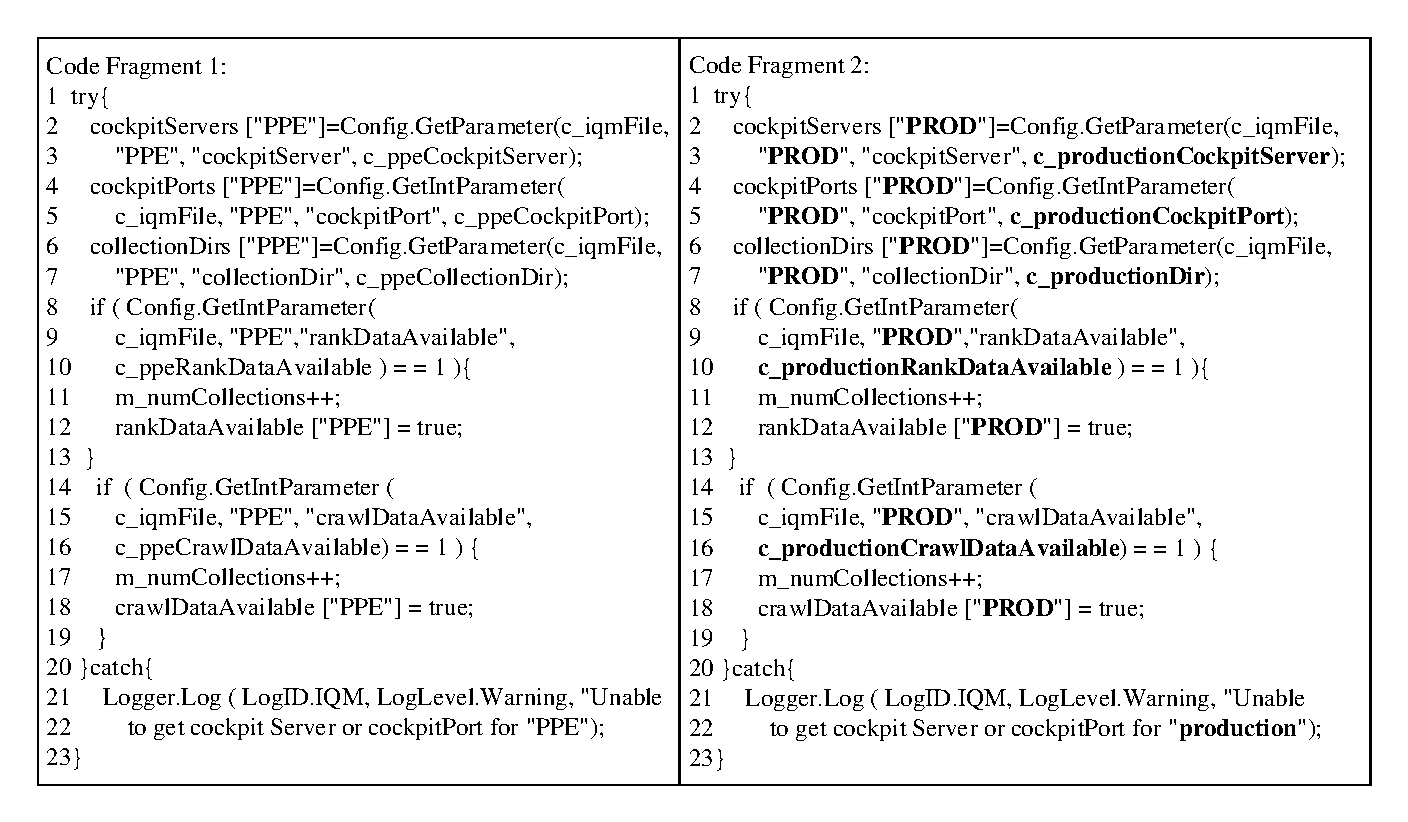
\includegraphics[width = 1.0\textwidth]{creatinga.pdf}
\bicaption[creatingexamplea]{}{会导致额外维护代价的克隆代码\cite{wang2014predicting}}
{Fig.$\!$}{An example for code fragments that resulting extra maintenance cost}
\vspace{-1em}
\end{figure}


但是并非所有的克隆代码都会导致额外的软件维护代价,图~\ref{creatingexampleb}~是不会导致额外维护代价的克隆代码。开发人员复制一段代码片段,并将其粘贴至其它位置。在引入此克隆代码后,该克隆代码一直安静的存在于系统中长达三年的时间,直到包含克隆代码的功能模块被移除。因此,对于此类复制粘贴所导致的克隆代码,并不会引发额外的维护代价。

\begin{figure}[htbp]
\centering
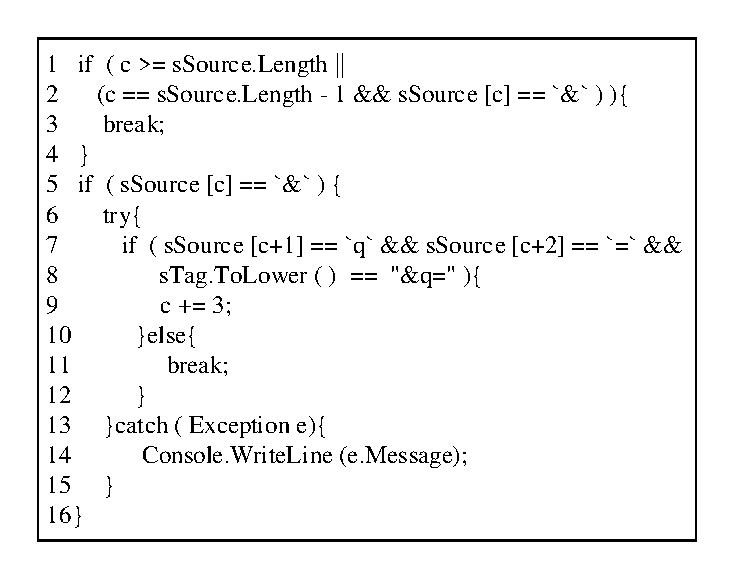
\includegraphics[width = 0.6\textwidth]{creatingb.pdf}
\bicaption[creatingexampleb]{}{不会导致额外维护代价的克隆代码\cite{wang2014predicting}}
{Fig.$\!$}{An example for code fragments that not resulting extra maintenance cost}
\vspace{-1em}
\end{figure}

\BiSubsection{现有方法存在的问题}
{Problems in Current Research}

在软件开发过程中,通过复制粘贴操作复用既有代码已经成为一种常见的软件开发手段\cite{koschke2007survey}。复用既有代码可以减少软件开发时间、提高软件开发效率,但同时也会向软件系统中引入大量的克隆代码。复制和粘贴导致的克隆代码可能引发额外的维护代价,如图~\ref{creatingexamplea}~所示。

针对克隆代码的维护代价问题,当前最主流的解决方式是使用重构的方法消除系统中的克隆代码。拟通过重构的手段消除克隆代码,进而避免克隆代码维护代价。目前的重构研究主要集中在可重构分析\cite{lin2014detecting,mende2009evaluation,schulze2008towards,choi2011extracting}、重构调度\cite{mandal2014automatic,lee2011automated,zibran2011constraint}、重构方法\cite{higo2008metric,krishnan2014unification,barbosa2013removing,ettinger2017efficient}等方面(见本文第~\ref{ref-clonerefactoring}~节克隆代码重构)。%但是,由于重构的代价较大,仅有少数的克隆代码适合于重构,因此无法解决克隆代码所导致的额外维护代价问题。

此外,为了有效地管理克隆代码,也对克隆代码进行跟踪,如跟踪新产生的克隆代码。由于复制粘贴操作是导致克隆产生的最主要原因,因此通过监测程序员的复制粘贴操作可以跟踪克隆代码的产生。例如,许多克隆跟踪工具CLONEBOARD\cite{de2009managing}、CnP\cite{hou2009cnp}、CPC\cite{weckerle2008cpc}、CReN\cite{jablonski2007cren}、CSeR\cite{jacob2010actively}等。但是,上述方法对新产生的克隆代码,并没有进行是否会导致额外维护代价的判断,而是将所有的克隆代码全部引入系统中。因此,也无法帮助降低克隆代码的额外维护代价。

目前对克隆代码研究无法有效地降低克隆代码的维护代价,依然存在以下两点不足:

(1)现有的克隆代码维护方法主要采用先检测后重构的方法,目标是消除克隆代码,而不是规避克隆代码的产生。这种基于重构的克隆代码维护方法不利于实现边开发边维护克隆代码,不能从源头上规避克隆代码的产生进而降低软件维护代价,而且重构本身的代价也很高,并非所有的克隆代码都适合重构,重构无法从根本上解决克隆代码的维护问题。

(2)在现有的克隆管理中的克隆代码跟踪研究中,通过跟踪复制粘贴操作跟踪克隆代码的产生,但是并未对复制粘贴操作加以控制,对这种操作是否会导致额外的维护代价缺少必要分析和判断。

综上,由于开发人员的复制粘贴操作会向系统中引入克隆代码,而克隆代码的一致性变化会导致额外的维护代价,这会降低软件系统的质量和可维护性。在软件开发过程中,帮助开发人员规避导致额外维护代价的克隆代码的产生,有助于降低克隆代码的额外的维护代价。因此,结合软件开发过程,在克隆代码创建时(复制和粘贴操作发生时),预测克隆代码的一致性维护需求是一个值得研究的问题,可以帮助规避会引入额外维护代价的克隆代码,从而降低软件的维护代价,提高软件质量和可维护性。%通过规避会导致额外维护代价的克隆代码产生,可以降低克隆代码的额外维护代价。通过允许不会导致额外维护代价的克隆代码的产生,可以提高软件开发效率。

\BiSubsection{本文的解决思路}
{The Proposed Method}

%%%因此,为了避免克隆代码的额外维护代价,可在克隆代码创建时的预测其一致性维护需求。Wang等人基于贝叶斯网络对克隆代码进行一致性维护需求预测研究\cite{wang2014predicting}。该方法中提取了历史属性、代码属性和上下文属性三组属性表示复制粘贴操作,取得了不错的预测效果。但是,该方法依然存在以下不足之处:
%%%
%%%\begin{itemize}
%%%\item
%%%首先,其所使用的历史属性与复制粘贴操作的关联性较弱,仅表示其所在文件的历史变化情况。同时历史属性的提取也增加了方法本身的困难程度(历史属性提取需要分析软件全部版本源代码);
%%%\item
%%%其次,所提取的代码属性和上下文属性不够充分,并不能完全的表示复制粘贴操作所导致的克隆代码。例如,代码属性中仅考虑了克隆代码与系统其它模块的调用和访问关系,并没有详细的考察克隆代码自身的一些属性特征。
%%%\item
%%%最后,方法中仅仅在贝叶斯网络上进行了实验,没有考虑其它机器学习方法的有效性。
%%%\end{itemize}

为了在克隆代码创建时避免其演化过程中可能导致的额外维护代价,本章将解决克隆一致性需求维护预测问题。在克隆代码演化的基础上,结合克隆代码一致性变化所导致的额外维护代价,给出了一种克隆代码创建时的一致性变化以及一致性维护需求的定义。定义不仅可以描述克隆代码所导致的维护代价,还将问题转化为一个可以使用机器学习方法可以解决的分类问题。然后,本文在Wang\cite{wang2014predicting}等人的研究基础上,改进了用于描述克隆代码的特征属性。舍弃了与复制粘贴操作关联性不强的历史属性,并进一步扩展了代码属性和上下文属性,可以更为细致地表示新创建的被复制和被粘贴的克隆代码。最后,使用五种不同的机器学习方法预测克隆代码创建的一致性维护需求。本章方法可以帮助程序开发人员降低克隆代码的一致性维护代价,提高软件的质量和可维护性。

本章的克隆代码创建一致性维护需求预测方法如图~\ref{framwork3}所示。从图中可以看出,该方法可以划分为三个阶段,复制和粘贴操作(克隆创建实例)收集阶段、特征提取阶段和一致性维护需求预测阶段。

收集阶段旨在收集系统中全部的复制和粘贴操作,将其用于使用机器学习方法中来训练预测模型。使用NiCad来检测软件版本中的所有克隆,并通过在相邻版本的克隆组之间进行映射来构建克隆家系,用于识别克隆创建实例。首先通过构建系统的克隆家系,然后,将第一次出现在系统的克隆代码标记为由复制和粘贴操作导致的克隆创建实例。最后,通过遍历系统全部克隆家系的根节点,可以收集系统所有的克隆创建实例。

由于实际的克隆创建实例无法直接应用于机器学习方法中,因此在特征提取阶段中将提取相应的属性特征表示克隆创建实例。分别提取了代码属性表示被复制的克隆代码,提取上下文属性表示被粘贴的克隆代码。

在预测步骤中,使用属性化的克隆创建实例构建和训练机器学习模型,并使用其预测克隆一致性维护需求。根据预测结果提醒程序开发人员采取进一步的操作。如果该复制和粘贴操作会导致一致性变化,程序开发人员可以据此拒绝此粘贴被复制的克隆代码,从而避免额外的维护代价。如果该复制粘贴操作不会导致一致性变化(不会引发额外的维护代价),程序开发人员可以放心的复用该克隆代码,从而提高软件开发的效率。

\begin{figure}[htbp]
\centering
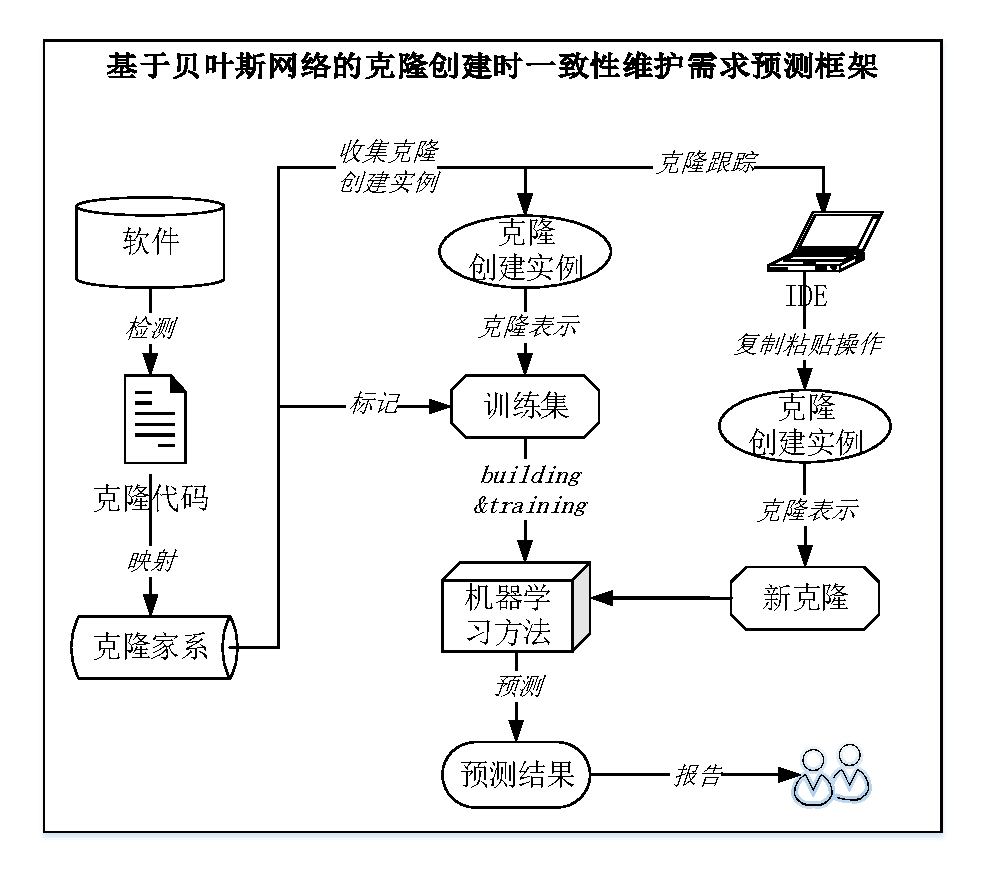
\includegraphics[width = 0.7\textwidth]{framework3.pdf}
\bicaption[framwork3]{}{克隆创建一致性维护需求预测方法}
{Fig.$\!$}{The approach for clone creating consistency prediction}
\vspace{-1em}
\end{figure}

本章在克隆代码创建时,预测克隆代码的一致性维护需求,本章将重点分析和讨论如下问题:

(1)在克隆代码创建时(复制和粘贴克隆代码时),结合其可能导致的额外维护代价,如何描述和定义其演化中的一致性变化与一致性维护需求?

(2)对于克隆创建实例(复制和被粘贴操作导致的克隆代码),如何进一步深入的描述和表示创建实例中的被复制的克隆代码和被粘贴的克隆代码?

(3)在预测克隆创建一致性维护需求时,如何结合软件开发过程,帮助程序开发人员避免额外的维护代价?
%该问题还可以划分为两个子问题:(a)不同的机器学习方法是否具有相似的预测能力?(b)并且所构建的模型对于两种不用的克隆创建实例,是否具有一致的预测能力?



\BiSection{克隆代码创建时一致性维护需求的定义}
{The Definitions for Clone Creating Consistency-Requirement}

如图~\ref{creatingexamplea}~所示,克隆代码的演化过程中,克隆代码可能会发生一致性变化,从而引发额外的维护代价。为了描述克隆代码所发生的变化,本文在第2章中给出了克隆代码的一致性变化模式,见定义\ref{def-evolutionpattern}。但是,
第2章所定义的克隆代码的一致性变化模式过于严格,无法直接将其用于描述克隆代码可能引发的额外维护代价。

在第2章的定义中,要求克隆组的所有克隆代码片段都要发生相同的变化,才称之为一致性变化。然而,本章的目标是避免克隆代码所导致额外的维护代价,当克隆组内的两个克隆代码同时发生变化时,同样会导致软件的额外维护代价。因此,在向系统中引入新的克隆代码时(克隆代码创建时),本章仅要求至少两个克隆代码片段同时发生变化。

因此,针对克隆代码所导致的额外维护代价问题,将克隆代码的一致性变化模式重新定义如下:

\begin{definition}[克隆创建时一致性变化模式] 
\label{def-creatingpattern}
在软件版本 $j+1$中存在一个克隆组$CG'$ ,假设克隆组内至少存在两个克隆代码片段$CF'_1$ 和 $CF'_2$可以与映射到上一版本$j$的克隆组$CG$中,且 $CG$中与之对应的克隆代码片段的 $(CF_1,CF_2)$被分别修改为$(CF'_1,CF'_2)$,满足
  \[
  \begin{array}[t]{cr}
    \mathit{TextSim}(CF_i, CF'_i) < 1 & \forall i \in \{1,2\}  \\
  \end{array}
  \]
则称克隆组$CG'$具有一致性变化模式(Consistent Change Pattern)。
\end{definition}

%在该定义中,克隆代码的变化使用$\mathit{TextSim}(CF_i, CF'_i)= 1 - UPI(CF_i, CF'_i)$描述。其中,UPI(Unique Percentage Items\cite{roy2008nicad})表示两个代码片段之间不同的代码行数占总代码行的比例。假如给定两个代码片段$CF_1$和$CF_2$,其$UPI(CF_1,CF_2)=0.3$表示两者的差异程度为30\%。同时,其相似度可根据$UPI$计算:$SimText (CF_1,CF_2)=1-UPI=0.7$,表示两者的相似度为70\%。

本章定义的克隆组的一致性变化模式,仅仅要求组内至少存在两个克隆代码片段被同时修改。对于一个克隆组来讲,组内至少存在两个克隆代码片段。假定要求组内全部的克隆代码片段都同时变化,为一致性变化模式。那么此种情况下的定义过于狭隘。原因在于:即使组内仅有两个克隆代码片段同时发生变化,即会导致额外的维护代价;而要求组内全部克隆片段全部同时变化,将无法准确的识别两个片段变化所所导致的维护代价。

如前文所述,系统中的大部分的克隆代码是由复制和粘贴操作所导致的。并且使用克隆家系还可以描述克隆代码的演化过程。因此,在一个克隆家系中,本文认定克隆家系的根节点就是克隆代码创建的时刻,根节点的克隆组是由程序开发人员的复制粘贴操作所创建的克隆代码(克隆创建实例)。因此,给出克隆创建实例的定义,如下所示:

\begin{definition}[克隆创建实例] 
\label{def-creatinginstance}
克隆创建实例:
软件版本 $j$中的一个克隆组$CG$是克隆创建实例,如果该克隆组$CG$是其克隆家系$CGE$的根节点,且该组的克隆代码是由复制粘贴操作引入的。
\end{definition}

给定一个由复制粘贴操作所创建的克隆组,在其演化过程中,可能会发生一致性变化,进而引发额外的维护代价。假设在创建该克隆代码时可以预测其是否可以发生一致性变化,可以避免额外的维护代价。因此,本文将由复制粘贴操作创建的克隆代码,其演化过程中发生的一致性变化,称为克隆创建一致性维护需求,定义如下:

\begin{definition}[克隆创建时一致性维护需求] 
 \label{def-creatingrequirement}
给定版本 $j$中一个克隆创建实例$CG$,如果在版本$k$中存在一个克隆组 $CG'$($k>j$)满足以下条件: (1) 在$CG'$中至少存在两个克隆片段在其克隆家系$CGE$中可以映射到克隆实例 $CG$中, (2) $CG'$ 具有“一致性变化模式”(Consistent Change Pattern),则称该克隆创建实例$CG$满足克隆创建的一致性维护需求(Consistency-Requirement);反之,假如不存在满足上述条件的克隆组$CG'$,则称 该克隆创建实例$CG$不满足克隆一致性维护需求(Consistency-Requirement Free,或Consistency-Free,或Free)。
\end{definition}

根据上面的定义描述,只要克隆代码在其演化过程中,发生过一致性变化模式,即认定其满足克隆一致性维护需求。最终,可以将本章的的研究问题可以表述如下:给定一个克隆创建实例$CG$,例如由复制粘贴操作导致的克隆代码,预测该创建实例$CG$是否满足克隆创建的一致性维护需求。

克隆创建实例只有两种状态:满足和不满足一致性维护需求。本章克隆创建的克隆一致性需求预测问题可转换为一个典型的分类问题,因此使用机器学习模型解决此分类问题。

\BiSection{复制和粘贴操作的样本获取}
{Collecting Copy-and-Paste Operations}
\label{lab-checkcopied}

根据定义~\ref{def-creatinginstance}~,本文假定克隆家系$CGE$中第一次出现的克隆代码是克隆创建实例,即复制粘贴操作导致的克隆代码。因此,通过检测系统的克隆代码并构建克隆家系,可以收集系统中的复制和粘贴操作。本章将使用NiCad来检测软件版本中的所有克隆。通过在相邻版本的克隆组之间进行映射来构建克隆家系。

(1)构建系统的克隆家系

首先,下载系统所有版本的源代码,并使用NiCad的默认配置检测检测每一版本的中Type1-3的克隆代码。然后,通过映射所有相邻版本的克隆代码,构建系统中全部克隆家系。为完成版本间的映射,为每个克隆片段生成一个克隆区域描述符 $CRD$\cite{duala2010clone},使用基于$CRD$的克隆映射算法映射两个连续版本之间的所有克隆片段和克隆组\cite{ci2013new,ci2013newD}。根据克隆映射结果,构建系统的克隆家系。

(2)收集复制粘贴操作并标识一致性维护需求

克隆家系是一个克隆组演化的有向无环图,图中根节点是由复制粘贴操导致的克隆创建实例。因此,根据定义~\ref{def-creatinginstance}~通过遍历克隆家系的根节点,可收集系统中所有的克隆创建实例,即复制和粘贴操作。在收集克隆创建实例的时候,同时根据定义~\ref{def-creatingpattern}~识别克隆一致性变化模式,从而确定克隆创建实例在其未来演化过程所发生的一致性变化。根据定义~\ref{def-creatingrequirement}~,如果克隆创建实例在其演化过程中发生了一致性变化模式(定义~\ref{def-creatingpattern}~),则该实例满足一致性维护需求,否则不满足维护需求。

(3)确认被复制和被粘贴的克隆代码

在收集克隆变化实例后,还需确认该实例中的被复制和被粘贴代码。由于被复制代码会较早地存在软件中,可将创建实例中的克隆代码向上一软件版本中进行映射。假定被复制代码会应存在于上一版本中,被粘贴代码不存在上版本中。根据映射结果,可能会存在两种情况:(a) 其中一个克隆代码可以映射,另一个未映射。认为映射代码为被复制代码,未映射为被粘贴代码。(b) 两者均没有映射。此情况下随机选取一个为被复制代码,另一个未未被粘贴代码。原因是两者互为克隆代码,彼此之间相似,故随机选取一个为被复制代码并不影响预测结果。注意不存在两者均可映射的情况,应在上一版本检测为克隆代码。\footnote{大多数克隆组只有两个克隆片段,所以这个决定不会影响我们的克隆预测。对于具有多个克隆片段的克隆组,则随机选取两个作为克隆创建实例。}

收集系统中复制和粘贴操作算法如~\ref{alg-collectioncreating}~所示。算法中第1-4行是为克隆代码生成CRD,并使用CRD映射相邻版本的克隆代码假设一个版本中有$m$个克隆代码,生成CRD所需时间为$O(m)$,$n$个版本所需时间为$O(m*n)$。映射克隆相邻版本的克隆代码时间复杂度为$O(m)$。算法的第5行为根据映射结果生成系统的克隆家系。第6-10行,先根据克隆创建实例定义,通过遍历克隆家系收集系统复制和粘贴操作。然后,根据克隆演化模式定义,识别克隆演化模式,并标记其一致性维护需求。最后,确认复制粘贴操作中被复制和被粘贴的克隆代码。算法复杂度为$O(n)$。所以,该算法的复杂度为$O(m*n)$。

\begin{minipage}{0.8\textwidth}
\centering
\begin{algorithm}[H]
\AlgoBiCaption{复制粘贴操作收集算法} {Algorithm for collecting copy-and-pasted operations}
\label{alg-collectioncreating}
\KwIn{All source code and code clones from $N$ versions}
\KwOut{All copy-and-paste operations}
\For{$i$=1 to $N$}
{ 
 Generating CRD to represent each code clone{CFs}\;
 Mapping all the $CFs$ and $CGs$ between the adjacent versions {i} and {i+1}\;
}
Generating all clone genealogies $CGEs$ with number $N\_cge$\;
\For{$i$=1 to $N\_cge$}
{ 
 Collecting the clone creating instance from $CGE\_i$ according to Definition~\ref{def-creatinginstance}~\; 
 Identify all clone consistent change pattern in thus two versions according to Definition~\ref{def-creatingpattern}~\;
 Labeling its consistency-requirement according to Definition~\ref{def-creatingrequirement}~; 
 Labeling the copied and pasted code fragments by mapping code clones to the last version\;
}
\Return {All copy-and-paste operations\;}
\end{algorithm}
\end{minipage}

\BiSection{复制粘贴操作的特征描述}
{The Attributes for Copied and Pasted Code Clones}
\label{lab-creatingattribute}

在使用机器学习中分类方法进行分类或者预测时,例如本章预测克隆代码创建的一致性维护需求,需要提前构建和训练机器学习模型。但是,实际的复制粘贴操作无法直接应用于机器学习中。

因此,本节将提取相应的属性值表示克隆创建实例(复制和粘贴操作)。一个克隆创建实例,即复制粘贴操作,由两个克隆代码片段构成:被复制的克隆代码代码和被粘贴的克隆代码。因此,本节将提取不同的属性用于描述复制和粘贴操作。提取代码属性表示被复制的克隆代码、提取上下文属性属性表示被粘贴的克隆代码。

\BiSubsection{被复制克隆代码的特征}
{The Attributes for the Copied Code Clone}

在克隆创建实例中,被复制的克隆代码代表系统中最初始的代码片段。因此,可以从代码本身的角度去描述被复制的克隆代码特征,即代码属性。代码属性描述克隆代码的词法、语法、函数调用等信息。代码属性主要包括克隆代码粒度、Halstead属性、结构属性、调用属性等,具体的代码属性如下所示:
%部分代码属性源于Wang的工作,本文在其基础上进行了扩展,新增Halstead度量属性、结构属性等。Halstead属性经常用于软件预测中,是用于描述代码特征的度量。结构属性是从代码的语法结构信息。

\begin{itemize}
\item 
克隆粒度:
被复制克隆代码的规模,即所包含的代码行数。
\item 
Halstead属性:
被复制克隆代码的代码复杂度,有四个基本的属性值,分别为操作符种类、操作数种类、操作符总量和操作数总量。
\item  
结构属性:
被复制克隆代码的结构特征,是语句的统计信息,{if\_then、if\_else、switch、while、do、for、this\_or\_super}等。
%被复制克隆代码的结构特征,是语句的统计信息,\verb+if_then+, \verb+if\_else+, \verb+switch+, \verb+while+, \verb+do+, \verb+for+,  \verb+this\_or\_super+等。
\item  
参数访问数量:
被复制克隆代码中所有函数的参数访问数量统计。
\item  
总函数调用次数:
被复制克隆代码中所有函数调用的次数统计。
\item  
本地函数调用次数:
被复制的克隆代码中,调用函数与被复制克隆片段在相同类的调用次数统计。
\item  
库函数调用次数:
被复制的克隆代码中,库函数的调用次数统计,包括java库函数的调用、eclipse库函数的调用以及第三方包函数的调用。
\item  
其它调用次数:
被复制的克隆代码中,既不是库函数调用、也不是本地函数调用的其它调用次数统计,如同项目内其它包函数调用或同包内其它类中的函数调用。
\end{itemize}

\BiSubsection{被粘贴克隆代码的特征}
{The Attributes for Pasted Code Clone}

对于克隆创建实例中的被粘贴的克隆代码,其包含了一些与克隆关系相关的特征,即上下文属性。上下文属性是代克隆创建实例中克隆代码之间的关系属性,描述了两者之间的克隆关系信息。上下文属性包括代码相似度、克隆分布、被复制和被粘贴代码之间的一些相似度等。
具体的上下文属性如下所示:
%部分上下文属性来自Wang的工作,同时本文也进行了扩展,新增代码相似度、参数类型相似度和块信息标识等属性。

\begin{itemize}
\item
代码相似度:
被复制与被粘贴的克隆代码之间的相似度,计算方法和NiCad相同,即UPI\cite{roy2008nicad}。
\item
局部克隆标识:
被复制及粘贴的克隆代码片段是否在同一个文件中。
\item
文件名相似度:
被复制和被粘贴克隆代码所在文件的名相似度。假定文件名分别为$M_1$和$M_2$,则文件名相似度为$Sim(M_1,M_2)$,采用李氏距离\cite{levenshtein1966binary,navarro2001guided}计算(剩余度量中相似度采用相同方法计算)。
\item
文件名相似度标识:
当克隆是局部克隆时,其文件名相似度为1,为非局部克隆时为0。该属性决定文件名相似度是否起效。
\item
方法名相似度:
被复制和被粘贴克隆代码所在方法的方法名字相似度。
\item
总参数名相似度:
假定被复制和被粘贴克隆代码所在方法为$M$和$N$,计算其参数名相似度之和。假设M和N分别包含m和n个参数,即$(P_1,P_2,…,P_m)$和$(Q_1,Q_2,…,Q_n)$,则总参数名相似度为$Sum(Sim(P_i,Q_j))$。
\item
最大参数名相似度:
假定被复制和被粘贴克隆代码所在方法为M和N,其最大参数名相似度。假设M和N分别包含m和n个参数,即$(P_1,P_2,…,P_m)$和$(Q_1,Q_2,…,Q_n)$,最大参数名相似度为$Max(Sim(P_i,Q_j))$。
\item 
总参数类型相似度:
被复制和被粘贴代码克隆所在方法分别为$M$和$N$,其参数类型相似度之和。假设$M$和$N$分别包含$m$和$n$个参数,其参数类型分别为$(P_1,P_2,…,P_m)$和$(Q_1,Q_2,…,Q_n)$,总参数类型相似度$Sum(Sim(P_i,Q_j))$。
\item
块信息标识:
被复制和被粘贴克隆代码的上下文信息是否相同,相同为$1$,反之为$0$。
\end{itemize}

\BiSection{基于机器学习的克隆创建一致性维护需求预测}
{Predicting Clone Creating Consistency-Requirement base on Machine Learning}
\label{lab-machine}

本章将克隆代码创建的一致性维护需求问题,转化成了克隆创建实例的分类问题,即给定一个克隆创建实例,判别其是否满足克隆创建的一致性维护需求。本章使用五种机器学习方法对克隆创建实例进行分类,从而预测克隆一致性维护需求。

在本章的研究中,使用五种不同的机器学习方法,即:贝叶斯网络方法(Bayesian Network,简写为BN)\cite{friedman1997bayesian,pearl1985bayesian}、朴素贝叶斯方法(Naive Bayes,简写为NB)\cite{john1995estimating},支持向量机方法(Support Vector Machine,简称为SVM)\cite{platt199912} 、K近邻方法(K-Nearest Neighbors,简写为KNN) \cite{aha1991instance}和决策树方法(Decision Tree,简写为DT)\cite{quinlan2014c4}。

(1)贝叶斯网络方法

贝叶斯网络是一种概率图型,可以使用已经观察到的事件来预测将来可能发生的事件\cite{friedman1997bayesian}。贝叶斯网络可以表示成一个有向无环图模型,图中的每一个节点表示一个随机事件,图中的边则表示随机事件发生的条件概率。因此, 贝叶斯网络中的全部节点可以视为一组随机变量{$X_{1},X_{2},...,X_{n}$},贝斯网络的边所有边则可以使用随机变量的条件概率表描述(Conditional Probability Distributions, CPD)。

一般而言,贝叶斯网络的节点可以是随机变量,可以是可观察到的变量、属性、未知参数等。连接两个贝叶斯网络节点的边则代表两个随机变量之间是非条件独立的,使用事件的条件概率表示。如果两个节点间没有连接,就称其随机变量彼此间为条件独立。条件概率表(CPT)可以描述贝叶斯网络的节点和边的因果关系。

对克隆代码一致性维护需求预测而言,贝叶斯网络可用来表示克隆创建实例的属性值及其一致性维护需求间的概率关系。克隆创建实例的属性值是贝叶斯网络中的随机事件。给定一个具体的克隆创建实例,可以使用贝叶斯网络计算该实例满足一致性维护需求的概率。

(2)朴素贝叶斯方法

朴素贝叶斯方法和贝叶斯网络类似,是运用贝叶斯定理为基础的简单概率分类器。但与贝叶斯网络不同的是,朴素贝叶斯方法的特征之间是强(朴素)独立的,因此称为朴素贝叶斯,即假定样本每个特征与其他特征都不相关。 

(3)支持向量机方法

支持向量机是另一种常见的机器学习方法,可以应用在分类与回归问题中。SVM模型将实例表示为空间中的点,并且试图构造一个超平面将不同类的实例(点)间隔开。更正式地来说,支持向量机在高维或无限维空间中构造超平面或超平面集合,可以用于分类问题中。直观来说,分类边界距离最近的训练数据点越远越好,因为这样可以缩小分类器的泛化误差。

以本文的克隆一致性需求分类为例,每一个克隆代码实例会抽象称为高维空间中的一个“点”,空间维数等同于所提取的属性数量。在使用SVM分类克隆实例时,将构造一个超平面分割开两种类别的克隆代码实例。

(4)K近邻方法

KNN方法是一种用于分类和回归的非参数统计方法。KNN是一种基于实例的学习方法,是局部近似和将所有计算推迟到分类之后的惰性学习。KNN会推迟对训练数据的建模,直到需要分类样本时才进行。在KNN分类中,输出是一个分类族群。一个实例的分类是由其邻居的“多数表决”确定的,K个最近邻居(k为正整数,通常较小)中最常见的分类决定了赋予该对象的类别。若k = 1,则该对象的类别直接由最近的一个节点赋予。邻居都取自一组已经正确分类(在回归的情况下,指属性值正确)的对象。

以本文克隆一致性预测为例,每一个克隆代码实例是KNN中的一个实例。在进行预测时,被预测的克隆实例的类别,将会有其最近的K个邻居进行表决,从而确定其一致性维护需求。

(5)决策树方法

机器学习中另一个常见的分类方法是决策树。决策树是一种简单但是广泛使用的分类器。通过训练数据构建决策树,可以高效的对未知的数据进行分类。决策树代表的是属性值与对象类别之间的一种映射关系。决策树是一个树结构(可以是二叉树或非二叉树)。树中每个节点表示某个属性,而每个分叉路径则代表的某个可能的权重,而每个叶结点则对应从根节点到该叶节点所经历的路径所表示的对象的类别。决策树仅有单一输出,若欲有复数输出,可以建立独立的决策树以处理不同输出。

以克隆一致性需求预测为例,克隆实例所提取的属性即是决策树中的属性,最后的克隆一致性维护需求则是对象的类别。

本章没有对机器学习方法进行改进和研究,模型的构建和训练通过调用现有机器学习工具包WEKA完成。WEKA(Waikato Environment for Knowledge Analysis)全称是怀卡托智能分析环境,它是一个Java语言编写的,支持数据挖掘任务的工作平台。WEKA集成了大量能承担数据挖掘任务的机器学习算法,包括数据预处理,分类,聚类,关联规则,特征选择以及可视化功能。

对于每个软件系统,首先,通过收集克隆创建实例并提取相应的属性,用于构建模型训练所需的数据集。然后,调用WEKA中的机器学习算法实现构建和训练克隆一致性预测模型。根据定义~\ref{def-creatingrequirement}~,克隆创建实例有两种不同的状态:需要一致性维护和不需要一致性维护:
\begin{itemize}
\item 
不需要一致性维护:
若克隆创建实例的预测结果为“不需要”,软件开发人员可以自由的执行克隆创建操作(复制和粘贴),从而节约开发时间提高开发效率。因为该克隆创建实例在未来演化的过程中不会引发一致性变化,也不会导致额外的维护代价。
\item
需要一致性维护:
若克隆创建实例的预测结果为“需要”,软件开发人员需要谨慎的执行克隆创建操作(复制和粘贴)。因为该克隆创建实例在未来演化的过程中可能会引发一致性变化,从而导致系统的额外维护代价。
\end{itemize}

基于机器学习的克隆创建一致性维护需求预测算法如~\ref{alg-creatingperdition}~所示。算法的第1行为初始化训练集。第2-6行提取相应的属性组表示克隆创建实例,并生成训练集。最后第7行,使用训练集调用WEKA训练机器学习模型。算法的主要时间消耗在表示克隆创建实例上,其时间复杂度为$O(m)$,其中m为复制粘贴操作的数量。

\begin{minipage}{0.8\textwidth}
\centering
\begin{algorithm}[H]
\AlgoBiCaption{克隆创建一致性维护需求预测算法} {Algorithm for predicting clone creating consistency}
\label{alg-creatingperdition}
\KwIn{All copy-and-paste operations and source code}
\KwOut{The predictive model}
Initializing the training data set $Sets$ for all the operations\; 
\For{$i$=1 to $M$} 
{ 
Generating all the code attributes for copied code clones\;
Generating all the context attributes for pasted code clones\;
Appending all the attributes as one item to the $Sets$\;
}
Calling WEKA to train the model on training set $Sets$\;
\Return {The predictive model\;}
\end{algorithm}
\end{minipage}

\BiSection{实验结果与分析}
{Experimental Results and Analysis}

\BiSubsection{实验设置}
{Experimental Methodology}

\BiSubsubsection{实验系统}
{Experimental Projects}

本章选取了四个Java开源软件进行实验,其中ArgoUML和 jEdit与第二章中所使用的系统相同。ArgoUML是一个领先的开源UML建模工具,jEdit是程序员开发所使用的编辑器。同时,新增两个新的系统,分别为jFreeChart和Tuxguitar。jFreeChart是一个开源Java库,可以帮助程序人员显示高质量的图表。Tuxguitar是一个多轨的吉他指法编辑器,可以使用其创建自己的吉他六线谱。

表~\ref{statisticsprojects}~给出了上述实验系统的基本信息,表中第2列给出了所使用系统的版本数量,第3-4列给出了系统的起始版本和结束版本。其中,选择14个版本的ArgoUML,22版本的jEdit,20个版本的jFreeChart和13个版本的Tuxguitar。

\begin{table}[htbp]
\bicaption [statisticsprojects]{}{四个开源软件实验系统信息}
{Table$\!$}{The information of four open sources experimental projects }
\vspace{0.5em}
\centering 
\wuhao
\begin{tabular}{cccc}
\toprule[1.5pt ]
{实验系统}&{版本数}&Start Version&End Version\\ 
\midrule[1pt]
ArgoUML&14&0.20.0&0.34.0\\ 
jEdit&22&3.0.0&5.0.0\\ 
jFreeChart&20&1.0.0&1.0.19\\ 
Tuxguitar&13&0.7.0&1.3.2\\ 
\bottomrule[1.5pt]
\end{tabular}
\end{table}

表~\ref{copysta}~给出了实验系统的克隆创建实例信息。其中,第2列和第3列列出了克隆创建实例的数量和比例,其中第2列是不需要一致性维护的实例,第3列是需要一致性维护实例的数量和比例。对于需要一致性维护的克隆创建实例,在其演化过程中可能导致一致性变化,从而增加系统维护代价。

从表~\ref{copysta}~中可以得出两个发现。第一,软件系统中存在大量的克隆创建实例,数量从633到3366,其中项目 jEdit是含有最少的克隆变化实例。这说明复用既有代码引入克隆代码,已经成为了程序开发人员的一种常用开发手段。第二,软件系统中大部分的克隆创建实例在其演化过程中不满足一致性维护要求(比例从59.8\%到88.47\%)。这表明作为一种常用开发手段的复制粘贴操作并不会在演化中引入一致的变化,这意味着开发人员可以正常的使用这种技术。

同时,还可以看出克隆代码在演化过程是比较稳定的,不易发生变化。这与本文第2章得出的克隆演化特征相一致。但是值得注意是:软件系统中依然存在相当数量的需要一致性维护的克隆创建实例,数量从73个到1353个。这也警告程序开发人员,即便可以使用复制粘贴复用已有代码,但也要注意克隆代码的一致性维护问题,不可以肆无忌惮的使用复用技术。

\begin{table}[htbp]
\bicaption[copysta]{}{实验系统的克隆创建实例信息统计}
{Table$\!$}{The statistics for clone creating instances in four projects}
\vspace{0.5em}
\centering
\wuhao
\begin{tabular}{cccc}
\toprule[1.5pt]
~\multirow{2}{*}{实验系统}& \multicolumn{2}{c}{克隆创建实例的数量(比例)} & \multirow{2}{*}{总数}\\ 
 \cline{2-3}
~&{不需要维护} &{需要维护} & ~\\
\midrule[1pt]
ArgoUML&	2574(77.07\%)&	766(22.93\%)&	3340\\
jEdit&	560(88.47\%)&	73(11.53\%)&	633\\
jFreeChart&	2013(59.80\%)&	1353(40.20\%)&	3366\\
Tuxguitar&	1016(71.10\%)&	413(28.90\%)&	1429\\
\bottomrule[1.5pt]
\end{tabular}
\end{table}

%我们在具有Intel(R)Core(TM)i5-4210M CPU @ 2.60GHz和8G RAM的桌面上运行我们的实验。每个实验花费不到一分钟的模型构建,交叉验证少于5分钟。大多数实验时间花费在数据准备,包括家谱建构和克隆变化实例收集,其范围在5至30分钟之间。然而,我们注意到,在实践中,克隆系谱构建和变更实例收集将逐步执行,随着软件发展到新版本。因此,数据准备的开销将不是实际问题。

为了详细评估本章所提出的克隆创建一致性维护需求预测方法,并回答本章所提出的两个子问题。本节实验可以划分为两个实验:有效性验证实验和使用模式实验,如下所示:
\begin{itemize}
\item
有效性验证实验(机器学习方法对比实验):在此实验中,使用五种不同机器学习方法验证本章方法的预测能力。可以帮助程序开发人员选择一个最优的机器学习模型,用于克隆代码创建的一致性维护需求预测。在此实验中,将同时预测两种类别的克隆创建实例。
\item
使用模式实验(贝叶斯网络方法实验):因为有两种不同类别的克隆创建实例,即需要一致性维护和不需要一致性维护。本节以贝叶斯网络方法为例,详细给出了两种状态下的具体预测结果。将分别预测两种类别的克隆创建实例,以帮助程序开发人员选择合适的“使用模式”进行克隆创建的一致性维护需求预测。
\end{itemize}

同时,本章提取了两组度量表示克隆创建实例,分别为代码属性和上下文属性。为了评估本章所提取的属性值的有效性,本章还将每一个实验进一步划分为全属性实验和属性组实验两个部分,如下所示:
\begin{itemize}
\item
全属性实验:在此实验中,使用本章所提取的所有属性进行预测实验,以评估本文方法的整体预测能力。
\item
属性组实验:
在此实验中,分别使用两组不同的属性值进行预测实验,以评估所提取的属性值对预测结果的影响程度。
\end{itemize}

\BiSubsubsection{实验评估指标}
{The Evaluation Metrics}
\label{ref-creatingmetrics}

在机器学习领域中,往往使用混淆矩阵(Confusion Matrix)描述一个模型的预测能力。混淆矩阵如表~\ref{confusion}~所示。在表中,True positives(TP)表示被正确地划分为正例的个数,即实际为正例且被分类器划分为正例的实例数。False positives(FP)表示被错误地划分为正例的个数,即实际为负例但被分类器划分为正例的实例数。False negatives(FN)表示被错误地划分为负例的个数,即实际为正例但被分类器划分为负例的实例数。True negatives(TN)表示被正确地划分为负例的个数,即实际为负例且被分类器划分为负例的实例数。  ​

\begin{table}[htbp]
\bicaption[confusion]{}{混淆矩阵示意图}
{Table$\!$}{The Confusion Matrix}
\vspace{0.5em}
\centering
\wuhao
\begin{tabular}{ccc}
\toprule[1.5pt]
~\multirow{2}{*}{真实类别}& \multicolumn{2}{c}{预测类别} ~\\ 
 \cline{2-3}
~&{类别$0$} &{类别$1$}~\\
\midrule[1pt]
类别$0$&True Positive(TP)	&False Negative(FN)\\
类别$1$&False Positive(FP)	&True Negative(TN)\\
\bottomrule[1.5pt]
\end{tabular}
\end{table}

根据混淆矩阵,使用计算精确率(Precision Rate)、召回率(Recall Rate)和F值(F-measure)用于评价模型的预测能力。对于类别$0$来说,其精确率可如下计算:
\begin{equation} 
\mbox{\it Precision}~=~{\frac {TP}{TP+FP}}
 \end{equation}
 
召回率可如下计算:
\begin{equation} 
\mbox{\it Recall}~=~{\frac {TP}{TP+FN}}
 \end{equation}

F-measure可如下计算:
\begin{equation} 
\mbox{\it F-measure} =2 \times {\frac {\mbox{\it precision} \times \mbox{\it recall} }{ \mbox{\it precision} + \mbox{\it recall} } }
 \end{equation}

在本章的一致性维护预测中,将同时预测两种不同的状态的创建实例的预测效果。首先,对于满足和不满足一致性维护需求的克隆创建实例,分别计算其精确率(Precision)、召回率(Recall)和F值(F-measure),用于评估不同类型实例的预测效果。然后,将这两组预测结果根据实际实例的数量进行加权平均,计算平均精确率(Average Precision)、平均召回率(Average Recall)和平均F值(Average F-measure)作为评价指标,计算方式如下所示:
\begin{itemize}
\item
平均精确率:
 该指标评估克隆创建实例的一致性维护需求预测的准确程度,包含了满足和不满足一致性维护需求的实例的预测。首先,计算预测中满足一致性维护需求的精确率``$P_1$'',即预测为满足一致性维护需求的克隆实例中正确预测的数量与全部预测数量的比值。然后,相似的计算不满足一致性维护需求的精确率``$P_2$''。最后,将这两个值进行加权平均,作为整个模型的精确率。 ``$P_1$'' 是满足一致性维护需求的精确率,并且训练集中所有满足一致性的实例数量为``$N_1$'' ;类似地, ``$P_2$''为不满足一致性维护需求的精确率,且 ``$N_2$''为其数量。平均精确率(Average Precision)计算如下,
\begin{equation} 
\mbox{\it Ave-Precision} ~=~ {\frac {P_1 \times N_1 + P_2 \times N_2}{N_1 + N_2}}
\end{equation}
\item
平均召回率:
该指标评估克隆创建实例的一致性维护预测的查全能力,也包含了满足求和不满足一致性维护需求的预测。同精确率,分别计算满足和不满足一致性维护需求的实例的召回率,然后对两者进行加权平均。“$R_1$” 是满足一致性维护需求的召回率,并且训练集中所有满足一致性的实例数量为“$N_1$” ;类似地,“$R_2$”为不满足一致性维护需求的召回率,且 “$N_2$”为实例数量。平均召回率(Average Recall)计算如下,
\begin{equation} 
\mbox{\it Ave-Recall} ~=~ {\frac  {R_1 \times N_1 + R_2 \times N_2}{N_1 + N_2}}.
\end{equation}

\item
平均F值:
该指标可以评估所有克隆创建实例的精确率和召回率的平均有效性。相似地,先分别计算满足和不满足一致性维护需求的克隆实例的F值,然后根据实例的数量进行加权平均。为计算本章预测的平均F-measure, ``$F_1$'' 是满足一致性维护需求的克隆实例的F值,且实例的个数为``$N_1$'';``$F_2$'' 是不满足一致性维护需求的克隆实例的F值,且实例的个数为``$N_1$'',则平均F值(Average F-measure) 可计算如下,
\begin{equation} 
\mbox{\it Ave-F-measure} ~=~ {\frac  {F_1 \times N_1 + F_2 \times N_2}{N_1 + N_2}}.
\end{equation}
\end{itemize}

\BiSubsection{有效性验证实验}
{The Effectiveness Experiments for Employed Machine Learning Methods}

在本节的实验中,讨论五种机器学习方法的预测能力,帮助程序开发人员选择合适的机器学习模型。因此,对每一个实验系统,同时使用五种不同的机器学习方法,同时对需要和不需要一致性维护的克隆实例进行预测。

值得注意的是,本章没有对机器学习方法本身做进一步的改进,直接调用WEKA中的机器学习算法进行评估和预测。在使用不同的机器学习方法时,需要对其进行一些基本的参数设置,以构建不同的机器学习模型。本文也没有对全部的参数进行调优,大多选择WEKA中默认的参数。通过调整机器学习的参数,可能进一步增强机器学习方法的预测能力。

所采用方法的参数设置如下:贝叶斯网络的父节点数设置为3,并且设置阈值为0.5。 朴素贝叶斯方法只有一个父节点,同样设置阈值为0.5。在支持向量机方法中,本章选择用{\em polynomial kernel\/}作为核函数。对决策树方法,采用了J48算法作为预测方法,并设置置信度为0.75。对K近邻方法,使用{\em Euclidean Distance\/}为距离函数,并且设置邻居个数为1。

在本节实验中,使用10-Folds Cross-Validity将数据集分为训练集和测试集,评估不同机器学习方法的预测能力。使用平均精确率(Average Precision)、平均召回率(Average Recall)和平均F值(Average F-measure)作为评价指标。采用五种不同的机器学习方法,预测克隆创建的克隆代码的一致性维护需求,实验分成了两个部分,分别为全属性实验和属性组实验,实验结果如表\ref{creatingallavg}~和~\ref{creatingsetavg}~所示。

\BiSubsubsection{全属性实验结果}
{The Results of Clone Creating Consistency for All Attributes}

表~\ref{creatingallavg}~给出了克隆创建实例的使用全部属性组的预测结果。从表中可以看出,五种不同的机器学习方法均可以高效地预测克隆一致性要求,精确率从79.3\%到95.8\%,召回率从79.4\%到95.8\% ,F值从79.4\%到95.7\%。

同时,对比不同机器学习方法的有效性,通过对比发现支持向量机在这四个实验系统上具有最佳的预测能力。具体来说,在系统 ArgoUML、jEdit和jFreeChart上有最好的结果。对于Tuxguitar系统来说,决策树具有最好的结果,SVM具有第二好的预测结果。与此同时,贝叶斯网络和朴素贝叶斯方法在这四个项目中几乎具有相对较差的预测结果,但是相差并不是特别明显。

因此,建议开发人员在需要预测克隆创建实例时首先考虑支持向量机,其它的机器学习方法也可以作为选择进行考虑。

\begin{table}[htbp]
\bicaption[creatingallavg]{}{克隆创建实例一致性维护需求预测效果}
{Table$\!$}{The effectiveness of clone creating consistency for all attribute}
\vspace{0.5em}
\centering
\wuhao
\begin{tabular}{cccccc}
\toprule[1.5pt]
{指标}&{方法}&{{ArgoUML}}&{{jEdit}}&{{jFreeChart}}&{{Tuxguitar}}\\
\midrule[1pt]
\multirow{5}{*}{平均Precision(\%)}
&{BN}&93.5&88.9&88.3&	83.1\\
&{NB}&	88.6&	87.1&	86.9&	79.3\\
&{SVM}&95.8&	92.4&90.6&88.8\\
&{KNN}&94&88.6&90&	84.8\\
&{DT}	&93.9&89.8	&89.3&88.9\\
\hline
\multirow{5}{*}{平均Recall(\%)}
&{BN}& 93.6&87.7&	88.2&	83.6\\
&{NB}&88.8&0.82&	86.8&79.4\\
&{SVM}& 95.8&92.1&90.4&88.3\\
&{KNN}&94&88.9&	90	&84.8\\
&{DT}&94	&90.5&	89.2&89.1\\
\hline
\multirow{5}{*}{平均F-measure(\%)}
&{BN}&93.5&88.2&88.1&83.2\\
&{NB}&88.7&84&86.7&79.4\\
&{SVM}&95.7&	90.3	&90.3&87.6\\
&{KNN}&94&88.7&	90	&	84.8\\
&{DT}	&93.9&	90.1	&89.2&89\\
\bottomrule[1.5pt]
\end{tabular}
\end{table}

%\begin{table}[htbp]
%\bicaption[creatingallfree]{}{克隆创建实例的一致性维护自由的预测效果}
%{Table$\!$}{The Effectiveness of Creating Instances for Consistency-Free}
%\vspace{0.5em}
%\centering
%\wuhao
%\begin{tabular}{cccccc}
%\toprule[1.5pt]
%{\textbf{Metric}}&{\textbf{Method}}&{\textbf{ArgoUML}}&{\textbf{jEdit}}&{\textbf{jFreeChart}}&{\textbf{Tuxguitar}}\\
%\midrule[1pt]
%\multirow{5}{*}{Precision}
%&{BN	}&0.945	&0.943	&0.879	&0.861\\
%&{Natvie	}&0.917	&0.941	&0.863	&0.853\\
%&{SVM}&	0.955	&0.919	&0.889	&0.872\\
%&{KNN}&	0.96	&0.933	&0.905&	0.891\\
%&{J48}&	0.953&	0.936	&0.891	&0.913\\
%\hline
%\multirow{5}{*}{Recall}
%&{BN}&	0.974&	0.916&	0.932	&0.917\\
%&{Natvie	}&0.94&	0.85&	0.927	&0.858\\
%&{SVM}&	0.992	&0.998	&0.959&	0.979\\
%&{KNN}&	0.962&	0.943	&0.93	&0.896\\
%&{J48}&	0.969&	0.959&	0.934&	0.935\\
%\hline
%\multirow{5}{*}{F-measure}
%&{BN}&	0.959	&0.929&	0.905&	0.888\\
%&{Natvie	}&0.928	&0.893	&0.894	&0.856\\
%&{SVM}&	0.973	&0.957&	0.923	&0.923\\
%&{KNN}&	0.961&	0.938	&0.917	&0.893\\
%&{J48}&     0.961&	0.947	&0.912&	0.924\\
%\bottomrule[1.5pt]
%\end{tabular}
%\end{table}

%\begin{table}[htbp]
%\bicaption[creatingallmeeting]{}{克隆创建实例的一致性维护需求的预测效果}{Table$\!$}
%{The Effectiveness of Creating Instances for Meeting Consistency-Requirement}
%\vspace{0.5em}
%\wuhao
%\centering
%\begin{tabular}{cccccc}
%\toprule[1.5pt]
%{\textbf{Metric}}&{\textbf{Method}}&{\textbf{ArgoUML}}&{\textbf{jEdit}}&{\textbf{jFreeChart}}&{\textbf{Tuxguitar}}\\
%\midrule[1pt]
%\multirow{5}{*}{Precision}
%&{BN}&	0.808	&0.575	&0.809	&0.637\\
%&{Natvie}&	0.714	&0.589	&0.78	&0.637\\
%&{SVM}&	0.845	&0.329	&0.823	&0.646\\
%&{KNN}&	0.864	&0.479	&0.854	&0.731\\
%&{J48}&	0.841	&0.493	&0.831	&0.782\\
%\hline
%\multirow{5}{*}{Recall}
%&{BN}&	0.902	&0.472	&0.889	&0.758\\
%&{Natvie}&	0.78	&0.339	&0.878	&0.646\\
%&{SVM}&	0.969	&0.96	&0.931	&0.927\\
%&{KNN}&	0.872	&0.522	&0.892	&0.74\\
%&{J48}&	0.891	&0.61	&0.894	&0.83\\
%\hline
%\multirow{5}{*}{F-measure}
%&{BN}&	0.853	&0.519	&0.847	&0.692\\
%&{Natvie}&	0.746	&0.43	&0.826	&0.641\\
%&{SVM}&	0.902	&0.49	&0.873	&0.762\\
%&{KNN}&	0.902	&0.49	&0.873	&0.762\\
%&{J48}&	0.865	&0.545	&0.861	&0.805\\
%\bottomrule[1.5pt]
%\end{tabular}
%\end{table}

\BiSubsubsection{属性组实验结果}
{The Results of Clone Creating Consistency for Attribute Set}

为了探索不同属性组对预测效果的影响,在五个机器学习方法上进行了属性组实验,实验结果如表~\ref{creatingsetavg}~所示。

从表中可以看出,属性组实验结果和全部属性组实验结果没有显着差异。这表明所使用的属性组不会对克隆创建时一致性预测产生负面影响。尽管如此,在全部实验结果中,效果最差的实验结果往往出现在属性组的实验结果中,即在仅使用代码属性或仅适用上下属属性预测时。具体来说,对系统ArgoUML、 jFreeChart和 Tuxguitar,其仅使用代码属性进行预测时五种机器学习方法的预测效果最差;而对系统jEdit仅仅使用“上下文” 属性的五种机器学习方法预测效果最差。

%最后,分析不同机器学习方法之间的预测能力,可以得出与全属性实验相似的结论,即五种机器学习方法的预测能力相差不大,但SVM方法具有相对最好的预测能力。因此建议程序开发人员在预测时保留所有的属性,并优先选择SVM方法。


\begin{table} [htbp]
\renewcommand\arraystretch{0.9} 
\bicaption[creatingsetavg]{}{克隆创建实例的属性组预测效果}
{Table$\!$}
{The effectiveness of attribute set for clone creating consistency}
\vspace{0.5em}
\centering
\wuhao
\begin{tabular}{cccccccc}
\toprule[1.5pt]
~{指标}&{实验系统}&{实验组}&{BN}&{NB}&{SVM}&{KNN}&{DT}~\\
\midrule[1pt]
\multirow{12}{*}{平均Precision(\%)}
&~\multirow{3}{*}{ArgoUML}
&全部属性& 93.5    & 88.6  &95.8 & 94  & 93.9 \\
& & 代码属性& 91.2    & 86.6  & 92.8 & 91.1 & 90.4 \\
&  & 上下文属性& 91.7    & 87.7  & 94.2 & 93.3 &93  \\
\cline{2-8}
&~\multirow{3}{*}{jEdit}
& 全部属性& 88.9    & 87.1  & 92.4 &88.6 & 89.8 \\
&    &代码属性& 88.5    & 86.5  & 92.4 & 90.3 & 88.2 \\
&    &  上下文属性 & 83     &83.2  & 90.9 & 87.7 & 87.6 \\
\cline{2-8}
&~\multirow{3}{*}{jFreeChart}
& 全部属性& 88.3    & 86.9  &90.6 &90  & 89.3 \\
&  &代码属性 & 80.8    & 75.5  & 81.9 & 80.8 & 80.2 \\
&  & 上下文属性& 90.3    & 87.3  & 90.6 & 89.8 & 89.1 \\
\cline{2-8}
&~\multirow{3}{*}{Tuxguitar} 
&全部属性 & 83.1    & 79.3  & 88.8 & 84.8 & 88.9 \\
&   &代码属性& 81.1    & 74.7  & 83.4 & 80.6 & 80   \\
&    &  上下文属性& 84.3    & 82.4  & 87.3 & 86.1 & 88.1 \\
\hline
\multirow{12}{*}{平均Recall(\%)}&
~\multirow{3}{*}{ArgoUML}
&全部属性 & 93.6    & 88.8  & 95.8 & 94  & 94  \\
&   &代码属性 & 91.4    & 86.8  & 92.9 & 91.2 & 90.5 \\
&   &  上下文属性& 91.9    & 88   & 94.3 & 93.4 & 93.1 \\
\cline{2-8}
&~\multirow{3}{*}{jEdit}
& 全部属性& 87.7    & 82   & 92.1 & 88.9 & 90.5 \\
&   &代码属性 & 86.9    & 83.6  & 92.1 & 91.2 & 89.6 \\
&   &  上下文属性& 85.2    & 82.6  & 91.8 & 88.5 & 88.9 \\
\cline{2-8}
&~\multirow{3}{*}{jFreeChart} 
 & 全部属性 & 88.2    & 86.8  & 90.4 & 90   & 89.2 \\
&  &代码属性 & 80.3    & 75.2  & 80.6 & 80.3 & 79.6 \\
&   &  上下文属性 & 90.3    & 87.3  & 90.4 & 89.8 & 89  \\
\cline{2-8}
&~\multirow{3}{*}{Tuxguitar} 
&全部属性 & 83.6    & 79.4  & 88.3 & 84.8 & 89.1 \\
&   &代码属性 & 81.7    & 75.6  & 83.7 & 81  & 80.7 \\
&    & 上下文属性& 84.6    & 81.6  & 87.4 & 86.2 & 88.2 \\
\hline
\multirow{12}{*}{平均F-measure(\%)}
&~\multirow{3}{*}{ArgoUML}
& 全部属性 & 93.5    & 88.7  & 95.7 & 94  & 93.9 \\
 &  & 代码属性 & 91.2    & 86.7  & 92.7 & 91.2 & 90.4 \\
 &   &  上下文属性& 91.7    & 87.8  & 94.1 & 93.3 & 93  \\
\cline{2-8}
&~\multirow{3}{*}{jEdit} 
& 全部属性 & 88.2    & 84   & 90.3 & 88.7 & 90.1 \\
&   &代码属性& 87.6    & 84.8  & 90.3 & 90.5 & 88.7 \\
&   &  上下文属性& 84     & 82.9  & 90.7 & 88.1 & 88.1 \\
\cline{2-8}
&~\multirow{3}{*}{jFreeChart} 
&  全部属性& 88.1    & 86.7  & 90.3 & 90   & 89.2 \\
&  &代码属性 & 79.7    & 74.1  & 79.7 & 79.6 & 78.8 \\
&   & 上下文属性 & 90.2    & 87.2  & 90.3 & 89.7 & 88.9 \\
\cline{2-8}
&~\multirow{3}{*}{Tuxguitar} 
&全部属性 & 83.2    & 79.4  & 87.6 & 84.8 & 89  \\
&  &代码属性& 81.1    & 75   & 82.7 & 80.7 & 80.2 \\
&  & 上下文属性& 84.4    & 81.9  & 86.9 & 86.2 & 88.1\\
\bottomrule[1.5pt]
\end{tabular}
\end{table} 

%%%%以下是未经转置的全部实验结果

%%%\begin{sidewaystable} [htbp]
%%%\bicaption[creatingsetavg]{}{克隆创建实例的属性组平均预测效果}
%%%{Table$\!$}
%%%{The average effectiveness of attribute set on creating instances for consistency}
%%%\vspace{0.5em}
%%%\centering
%%%\wuhao
%%%\begin{tabular}{cccccccccccccc}
%%%\toprule[1.5pt]
%%%\multirow{2}{*}{指标}&\multirow{2}{*}{方法}&\multicolumn{3}{c}{ArgoUML}&\multicolumn{3}{c}{jEdit}&\multicolumn{3}{c}{jFreeChart}&\multicolumn{3}{c}{Tuxguitar}\\
%%%\cline{3-14}
%%%&&{全部}&{代码}&{上下文}&{全部}&{代码}&{上下文}&{全部}&{代码}&{上下文}&{全部}&{代码}&{上下文}~\\
%%%\midrule[1pt]
%%%\multirow{5}{*}{平均Percision}
%%%&BN&	0.935&	0.912&	0.917&		0.889&	0.885&	0.83&		0.883&	0.808&	0.903&		0.831&	0.811&	0.843\\
%%%&NB&	0.886&	0.866&	0.877&		0.871&	0.865&	0.832&		0.869&	0.755&	0.873&		0.793&	0.747&	0.824\\
%%%&SVM&	0.958&	0.928&	0.942&		0.924&	0.924&	0.909&		0.906&	0.819&	0.906&		0.888&	0.834&	0.873\\
%%%&KNN&	0.94&	0.911&	0.933&		0.886&	0.903&	0.877&		0.9	&0.808&	0.898&		0.848&	0.806&	0.861\\
%%%&DT&	0.939&	0.904&	0.93&		0.898&	0.882&	0.876&		0.893&	0.802&	0.891&		0.889&	0.8&	0.881\\
%%%\hline
%%%\multirow{5}{*}{平均Recall}
%%%&BN&	0.936&	0.914&	0.919&		0.877&	0.869&	0.852&		0.882&	0.803&	0.903&		0.836&	0.817&	0.846\\
%%%&NB&	0.888&	0.868&	0.88&		0.82&	0.836&	0.826&		0.868&	0.752&	0.873&		0.794&	0.756&	0.816\\
%%%&SVM&	0.958&	0.929&	0.943&		0.921&	0.921&	0.918&		0.904&	0.806&	0.904&		0.883&	0.837&	0.874\\
%%%&KNN&	0.94&	0.912&	0.934&		0.889&	0.912&	0.885&		0.9&	0.803&	0.898&		0.848&	0.81&	0.862\\
%%%&DT&	0.94&	0.905&	0.931&		0.905&	0.896&	0.889&		0.892&	0.796&	0.89&		0.891&	0.807&	0.882\\
%%%\hline
%%%\multirow{5}{*}{平均F-measure}
%%%&BN&	0.935&	0.912&	0.917&		0.882&	0.876&	0.84&		0.881&	0.797&	0.902&		0.832&	0.811&	0.844\\
%%%&NB&	0.887&	0.867&	0.878&		0.84&	0.848&	0.829&		0.867&	0.741&	0.872&		0.794&	0.75&	0.819\\
%%%&SVM&	0.957&	0.927&	0.941&		0.903&	0.903&	0.907&		0.903&	0.797&	0.903&		0.876&	0.827&	0.869\\
%%%&KNN&	0.94&	0.912&	0.933&		0.887&	0.905&	0.881&		0.9&	0.796&	0.897&		0.848&	0.807&	0.862\\
%%%&DT&	0.939&	0.904&	0.93&		0.901&	0.887&	0.881&		0.892&	0.788&	0.889&		0.89&	0.802&	0.881\\
%%%\bottomrule[1.5pt]
%%%\end{tabular}
%%%\end{sidewaystable} 

%\begin{sidewaystable} [htbp]
%\bicaption[creatingsetfree]{}{克隆创建实例的属性组克隆一致性维护自由预测效果}{Table$\!$}
%{The Effectiveness of Attribute Set on Creating Instances for Consistency-Requirement Free}
%\vspace{0.5em}
%\centering
%\wuhao
%\begin{tabular}{cccccccccccccc}
%\toprule[1.5pt]
%\multirow{2}{*}{\textbf{Metric}}&\multirow{2}{*}{\textbf{Method}}&\multicolumn{3}{c}{\textbf{ArgoUML}}&\multicolumn{3}{c}{\textbf{jEdit}}&\multicolumn{3}{c}{\textbf{jFreeChart}}&\multicolumn{3}{c}{\textbf{Tuxguitar}}\\
%\cline{3-14}
%&&\textbf{All}&\textbf{Code}&\textbf{Context}&\textbf{All}&\textbf{Code}&\textbf{Context}&\textbf{All}&\textbf{Code}&\textbf{Context}&\textbf{All}&\textbf{Code}&\textbf{Context}~\\
%\midrule[1pt]
%\multirow{5}{*}{Precision}
%&BN&0.945&	0.932	&0.929&		0.943&	0.942	&0.9	&	&0.879	&0.789	&0.898		&0.861	&0.848	0.88\\
%&NB&0.917	&0.907&	0.913	&	0.941	&0.932&	0.906	&	0.863&	0.744&	0.873	&	0.853&	0.809	&0.89\\
%&SVM&0.955&	0.937	&0.945	&	0.919	&0.919&	0.928&		0.889	&0.779&	0.889	&	0.872	&0.843	&0.877\\
%&KNN&0.96	&0.94	&0.947	&	0.933&	0.934	&0.926	&	0.905&	0.787&	0.896	&	0.891&	0.856&	0.9\\
%&DT&0.953&	0.936	&0.943	&	0.936&	0.923	&0.921&		0.891&	0.778&	0.884	&	0.913	&0.842&	0.907\\
%
%\hline
%\multirow{5}{*}{Recall}
%&BN&0.974	&0.958	&0.969	&	0.916	&0.907&	0.936		&0.932	&0.916	&0.944	&	0.917	&0.905	&0.906\\
%&NB&0.94	&0.924	&0.933&		0.85	&0.879&	0.896		&0.927&	0.892	&0.922	&	0.858	&0.86&	0.845\\
%&SVM&0.992	&0.973&	0.983		&0.998	&0.998&	0.984		&0.959	&0.944	&0.959		&0.979	&0.947	&0.957\\
%&KNN&0.962&	0.946&	0.969	&	0.943	&0.968&	0.945		&0.93&	0.919&	0.937	&	0.896	&0.881&	0.907\\
%&DT&0.969&	0.941	&0.969	&	0.959&	0.963	&0.957	&	0.934	&0.92&	0.939	&	0.935	&0.897	&0.93\\
%\hline
%\multirow{5}{*}{F-measure}
%&BN&0.959&	0.945&	0.949	&	0.929	&0.924&	0.918	&	0.905&	0.848	&0.921	&	0.888&	0.875&	0.893\\
%&NB&0.928&	0.915	&0.923	&0.893	&0.904	&0.901		&0.894&	0.811&	0.897	&	0.856	&0.834	&0.867\\
%&SVM&0.973&	0.955&	0.964	&	0.957&	0.957&	0.955	&	0.923&	0.854	&0.923&		0.923&	0.892&	0.915\\
%&KNN&0.961&	0.943&	0.958	&	0.938	&0.951&	0.935		&0.917	&0.848	&0.916&		0.893&	0.868	&0.903\\
%&DT&0.961&	0.938&	0.956	&	0.947	&0.942&	0.939	&	0.912&	0.843	&0.911&		0.924	&0.868&	0.918\\
%\bottomrule[1.5pt]
%\end{tabular}
%\end{sidewaystable}

%\begin{sidewaystable} [htbp]
%\footnotesize
%\bicaption[sdfj1]{}{克隆创建实例的属性组克隆一致性维护自由预测效果}{Table$\!$}
%{The Effectiveness of Attribute Set for Creating Instances for Meeting Consistency-Requirement}
%\vspace{0.5em}
%\centering
%%\wuhao
%\begin{tabular}{cccccccccccccc}
%\toprule[1.5pt]
%\multirow{2}{*}{\textbf{Metric}}&\multirow{2}{*}{\textbf{Method}}&\multicolumn{3}{c}{\textbf{ArgoUML}}&\multicolumn{3}{c}{\textbf{jEdit}}&\multicolumn{3}{c}{\textbf{jFreeChart}}&\multicolumn{3}{c}{\textbf{Tuxguitar}}\\
%\cline{3-14}
%&&\textbf{All}&\textbf{Code}&\textbf{Context}&\textbf{All}&\textbf{Code}&\textbf{Context}&\textbf{All}&\textbf{Code}&\textbf{Context}&\textbf{All}&\textbf{Code}&\textbf{Context}~\\
%\midrule[1pt]
%\multirow{5}{*}{Precision}
%&BN&	0.902	&0.844	&0.878	&	0.472	&0.447	&0.294	&	0.889	&0.836	&0.91	&	0.758	&0.719	&0.752\\
%&NB&	0.78&	0.728&	0.756	&	0.339	&0.352	&0.266	&	0.878	&0.772	&0.873	&	0.646	&0.593	&0.662\\
%&SVM&	0.969	&0.896	&0.934	&	0.96	&0.96&	0.769	&	0.931	&0.879	&0.931	&	0.927&	0.813	&0.863\\
%&KNN&	0.872	&0.815	&0.888		&0.522	&0.66	&0.5		&0.892	&0.839	&0.9	&	0.74&	0.684	&0.767\\
%&DT&	0.891	&0.799&	0.885	&	0.61	&0.571	&0.529	&	0.894	&0.837&	0.901	&	0.83	&0.697	&0.817\\
%\hline
%\multirow{5}{*}{Recall}
%&BN&	0.808	&0.765&	0.752		&0.575	&0.575	&0.205	&	0.809&	0.636&	0.841	&	0.637&	0.6	&0.697\\
%&NB&	0.714&	0.68	&0.701	&	0.589	&0.507&	0.288		&0.78	&0.542	&0.8	&	0.637	&0.501	&0.743\\
%&SVM&	0.845&	0.779	&0.808	&	0.329	&0.329&	0.411	&	0.823	&0.601&	0.821	&	0.646	&0.567	&0.671\\
%&KNN&	0.864&	0.798	&0.816	&	0.479	&0.479&	0.425	&	0.854&	0.63&	0.838		&0.731	&0.634&	0.751\\
%&DT&	0.841&	0.782	&0.803	&	0.493	&0.384&	0.37	&	0.831&	0.61&	0.817	&	0.782	&0.586	&0.765\\
%\hline
%\multirow{5}{*}{F-measure}
%&BN&	0.853&	0.803&	0.81	&	0.519	&0.503&	0.242	&	0.847&	0.722&	0.874	&	0.692&	0.654&	0.724\\
%&NB&	0.746&	0.703	&0.728		&0.43	&0.416	&0.276	&	0.826	&0.637	&0.835		&0.641	&0.543	&0.7\\
%&SVM&	0.902&	0.834&	0.866&		0.49&	0.49	&0.536	&	0.873&	0.714	&0.873	&	0.762	&0.668&	0.755\\
%&KNN&	0.868&	0.806&	0.85	&	0.5&	0.556	&0.459		&0.873	&0.72	&0.868		&0.736&	0.658	&0.759\\
%&DT&	0.865&	0.79&	0.842	&	0.545&	0.459&	0.435	&	0.861	&0.706&	0.857	&	0.805	&0.637&	0.79\\
%\bottomrule[1.5pt]
%\end{tabular}
%\end{sidewaystable}

\BiSubsection{使用模式实验}
{The Experiments for Two Usage Scenarios}

本节以贝叶斯网络方法为例,分别预测两种不同类别的克隆创建实例,即不满足一致性维护需求实验(一致性维护自由实验)和满足一致性维护需求实验。在构建贝叶斯网络时,使用 K2算法建立网络结构,并设置贝叶斯网络的最大父节点个数为3,同时使用SimpleEstimator估计贝叶斯网络的条件概率表。在实验时,采用十倍交叉验证(10-Folds Cross-Validity)将克隆创建实例的数据集划分为训练集和测试集,并评估预测模型的预测能力。

使用贝叶斯网络方法进行预测时,会计算克隆创建实例的概率值,表示该实例需要一致性维护需求的概率(在0-1之间,数值接近于1表示需要一致性维护,接近于0表示不需要一致性维护)。针对不同的克隆创建实例,设置了不同的阈值进行实验分析。对于不需要一致性维护的实例,其预测值较小(接近于0),当预测值小于等于给定阈值时认定该实例不需要一致性维护。对于需要一致性维护的实例,其贝叶斯网络预测值较大(接近于1),当预测值大于等于该阈值认定该实例需要一致性维护。

\BiSubsubsection{一致性维护自由实验}
{The Experiment for Clone Creating Consistency-Free}

对不需要一致性维护的克隆创建实例进行预测评估,可以帮助程序开发人员执行复制和粘贴操作,从而快速安全的开发软件。实验使用三个度量评估预测效果,分别为:推荐率、精确率和召回率。其中,推荐率(Recommendation Rate)指的是所推荐的不需要一致性维护的克隆创建实例比例,即预测为不需要一致性维护的克隆创建实例与系统中全部实例的比值。

%%%\begin{itemize}
%%%\item	
%%%推荐率(Recommendation Rate):指的是所推荐的不需要一致性维护的克隆创建实例比例,即预测为不需要一致性维护的克隆创建实例与系统中全部实例的比值。
%%%\item  
%%%精确率(Precision Rate):指所预测的不需要一致性维护复制粘贴实例的精确率,即在预测为不需要一致性维护的复制粘贴实例中,正确预测的实例与所预测实例的比值。
%%%\item  
%%%召回率(Recall Rate):指所推荐的不需要一致性维护的复制粘贴实例的查全率,即预测为不需要一致性维护的复制粘贴实例,与系统中的不需要一致性维护的实例的比值。
%%%\end{itemize}

(1)全属性实验结果

全属性实验同样使用全部属性在四个实验系统上进行评估,实验结果如图~\ref{creatingallfree}~所示。

\begin{figure}[h]
\centering
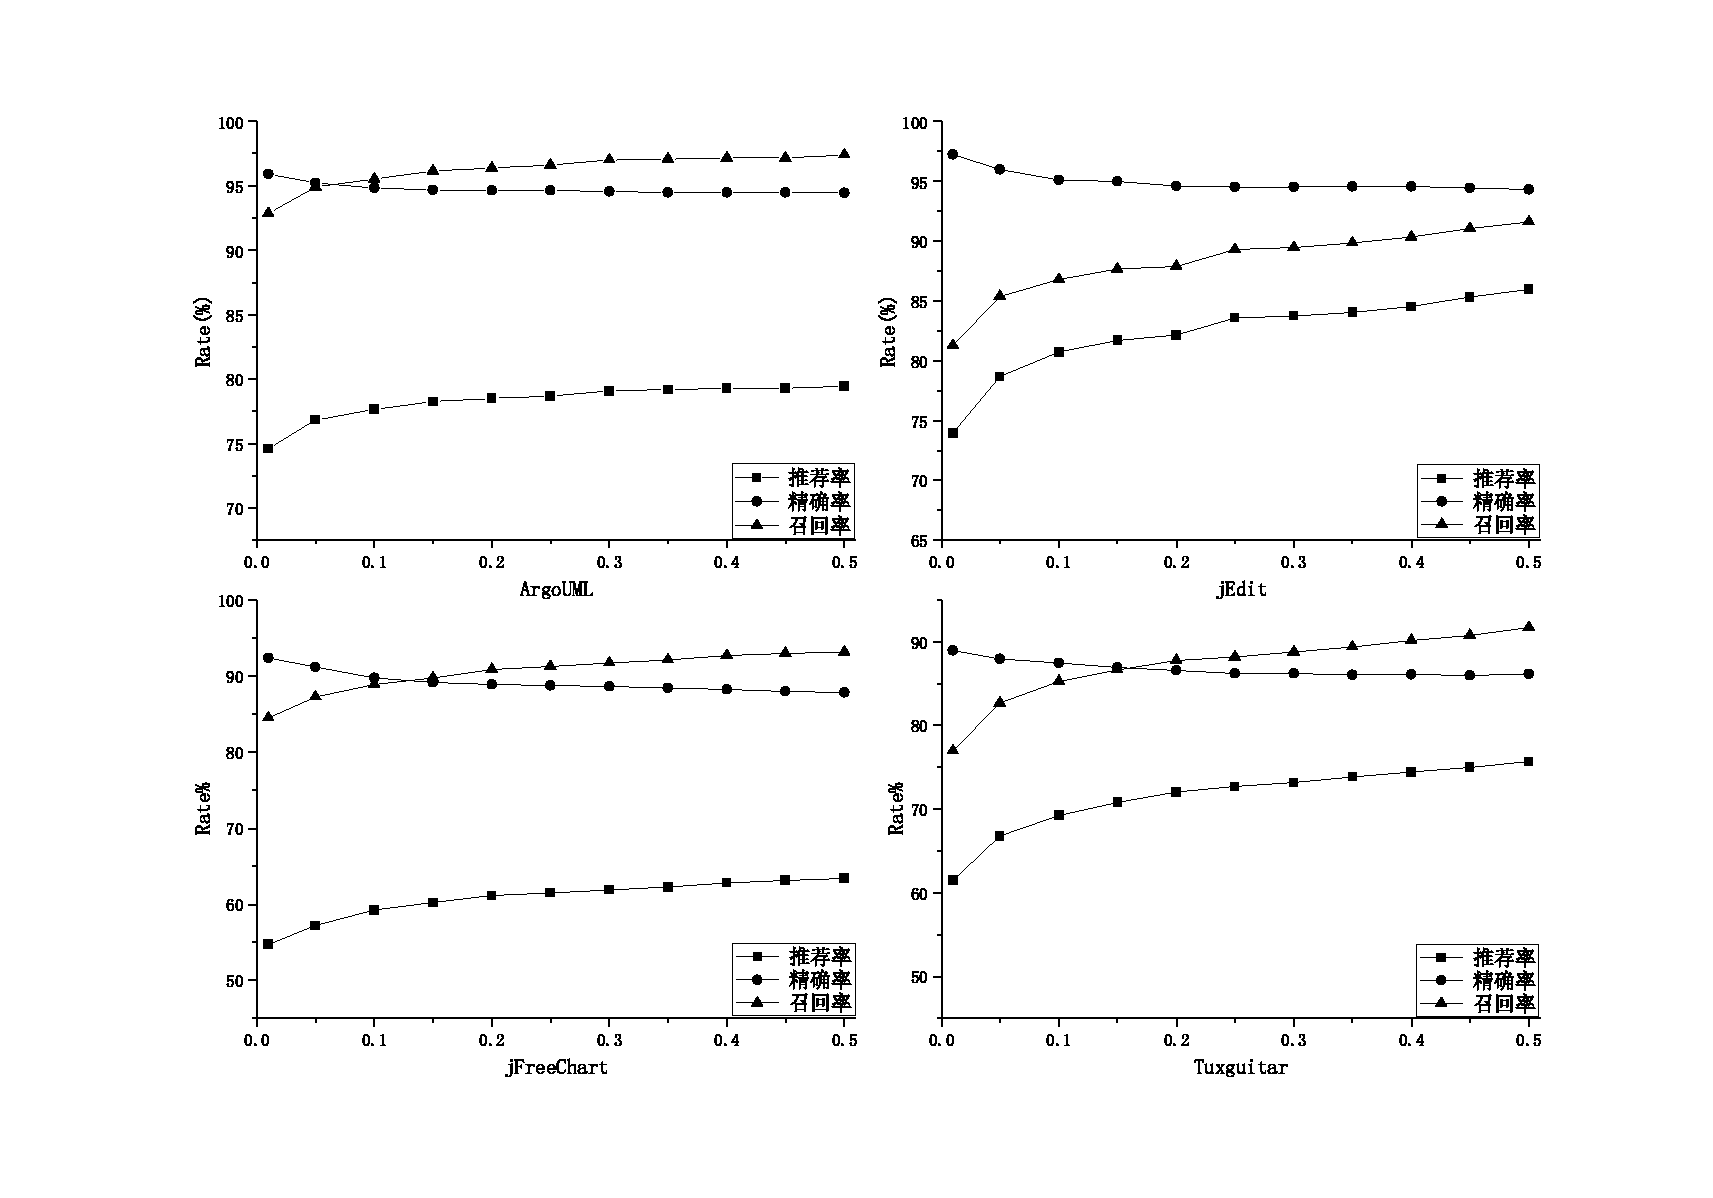
\includegraphics[width = 1.0\textwidth]{bayesgraph/creatingallfree.pdf}
\bicaption[creatingallfree]{}{全属性组维护自由实验效果}
{Fig.$\!$}{The effectiveness for all attribute of clone consistency free}
\vspace{-1em}
\end{figure}

由图中可以看出,本文方法在预测不需要一致性维护的克隆创建实例时,在四个系统上均取得了较好效果。根据预测结果,四个系统的精确率介于86.2\% -- 97.2\%之间,同时召回率也达到较高值,介于77\% -- 97.4\%之间。

由图~\ref{creatingallfree}~和表~\ref{copysta}~中可以看出,本文的推荐率达到了一个合理的水平, 和系统中不需要一致性维护的克隆实例比例相差不大。同时,阈值对预测结果的影响不大,准确度会随着阈值的降低而缓慢增大。四个系统在不同的阈值的准确度均较高。

因此,在使用全部属性预测不需要一致性维护的克隆创建实例时,可以达到一个较好的预测效果。


%%%%全属性实验同样使用全部属性在四个实验系统上进行评估,实验结果如表~\ref{copyallfree}~所示。由表中可以看出,本文方法在预测不需要一致性维护的克隆创建实例时,在四个系统上均取得了较好效果。根据预测结果,四个系统的精确率介于86.6--97.22\%之间,同时召回率也达到较高值,介于76.97--96.39\%之间。由表~\ref{copyallfree}~和表~\ref{copysta}~中可以看出,本文的推荐率达到了一个合理的水平, 和系统中不需要一致性维护的克隆实例比例相差不大。同时,阈值对预测结果的影响不大,准确度会随着阈值的降低而缓慢增大。四个系统在不同的阈值的准确度均较高。
%%%%
%%%%因此,本章方法在使用全属性在贝叶斯网络作为分类器时,可以达到一个较好的预测效果。

%%%%%五个阈值的实验表
%%%%%\begin{table}[htbp]
%%%%%\bicaption[copyallfree]{}{全属性组维护自由实验效果}
%%%%%{Table$\!$}{The effectiveness for all attribute of clone consistency free}
%%%%%\vspace{0.5em}
%%%%%\centering
%%%%%\wuhao
%%%%%\begin{tabular}{ccccc}
%%%%%\toprule[1.5pt]
%%%%%{系统}&{阈值}&{推荐率(\%)}&{精确率(\%)}&{召回率(\%)}\\
%%%%%\midrule[1pt]
%%%%%\multirow{5}{*}{ArgoUML}
%%%%%&0.01&	74.61&	95.91&	92.85\\
%%%%%&0.05&	76.83&	95.21&	94.91\\
%%%%%&0.1&	77.63&	94.83&	95.53\\
%%%%%&0.15&  78.26&	94.68&	96.15\\
%%%%%&0.2&	78.47&	94.66&	96.39\\
%%%%%\hline
%%%%%\multirow{5}{*}{jEdit}
%%%%%&0.01&	73.93&	97.22&	81.25\\
%%%%%&0.05&	78.67&	95.98&	85.36	\\
%%%%%&0.1&	80.73&	95.11&	86.79	\\
%%%%%&0.15&	81.67&	94.97&	87.68	\\
%%%%%&0.2&	82.15&	94.62&	87.86	\\
%%%%%\hline
%%%%%\multirow{5}{*}{jFreeChart}
%%%%%&0.01&	54.69&	92.40&	84.50\\
%%%%%&0.05&	57.22&	91.23&	87.28\\
%%%%%&0.1&	59.24&	89.72&	88.87\\
%%%%%&0.15&	60.22&	89.15&	89.77\\
%%%%%&0.2&	61.14&	88.87&	90.86\\
%%%%%\hline
%%%%%\multirow{5}{*}{Tuxguitar}
%%%%%&0.01&	61.51&	88.96&	76.97\\
%%%%%&0.05&	66.83&	87.96&	82.68\\
%%%%%&0.1&	69.28&	87.47&	85.24\\
%%%%%&0.15&	70.82&	86.96&	86.61\\
%%%%%&0.2&	72.08&	86.60&	87.80\\
%%%%%\bottomrule[1.5pt]
%%%%%\end{tabular}
%%%%%\end{table}

(2)属性组实验

实验结果如图~\ref{creatingsetfree}~所示,其中使用“RR”表示推荐率,“P”表示精确率,“R”表示召回率。并同时使用不同的后缀表示不同属性组的实验结果,其中“All”为全属性组实验结果,“Code”表示仅使用代码属性的实验结果,“Context”表示上下文属性的实验结果。

\begin{figure}[h]
\centering
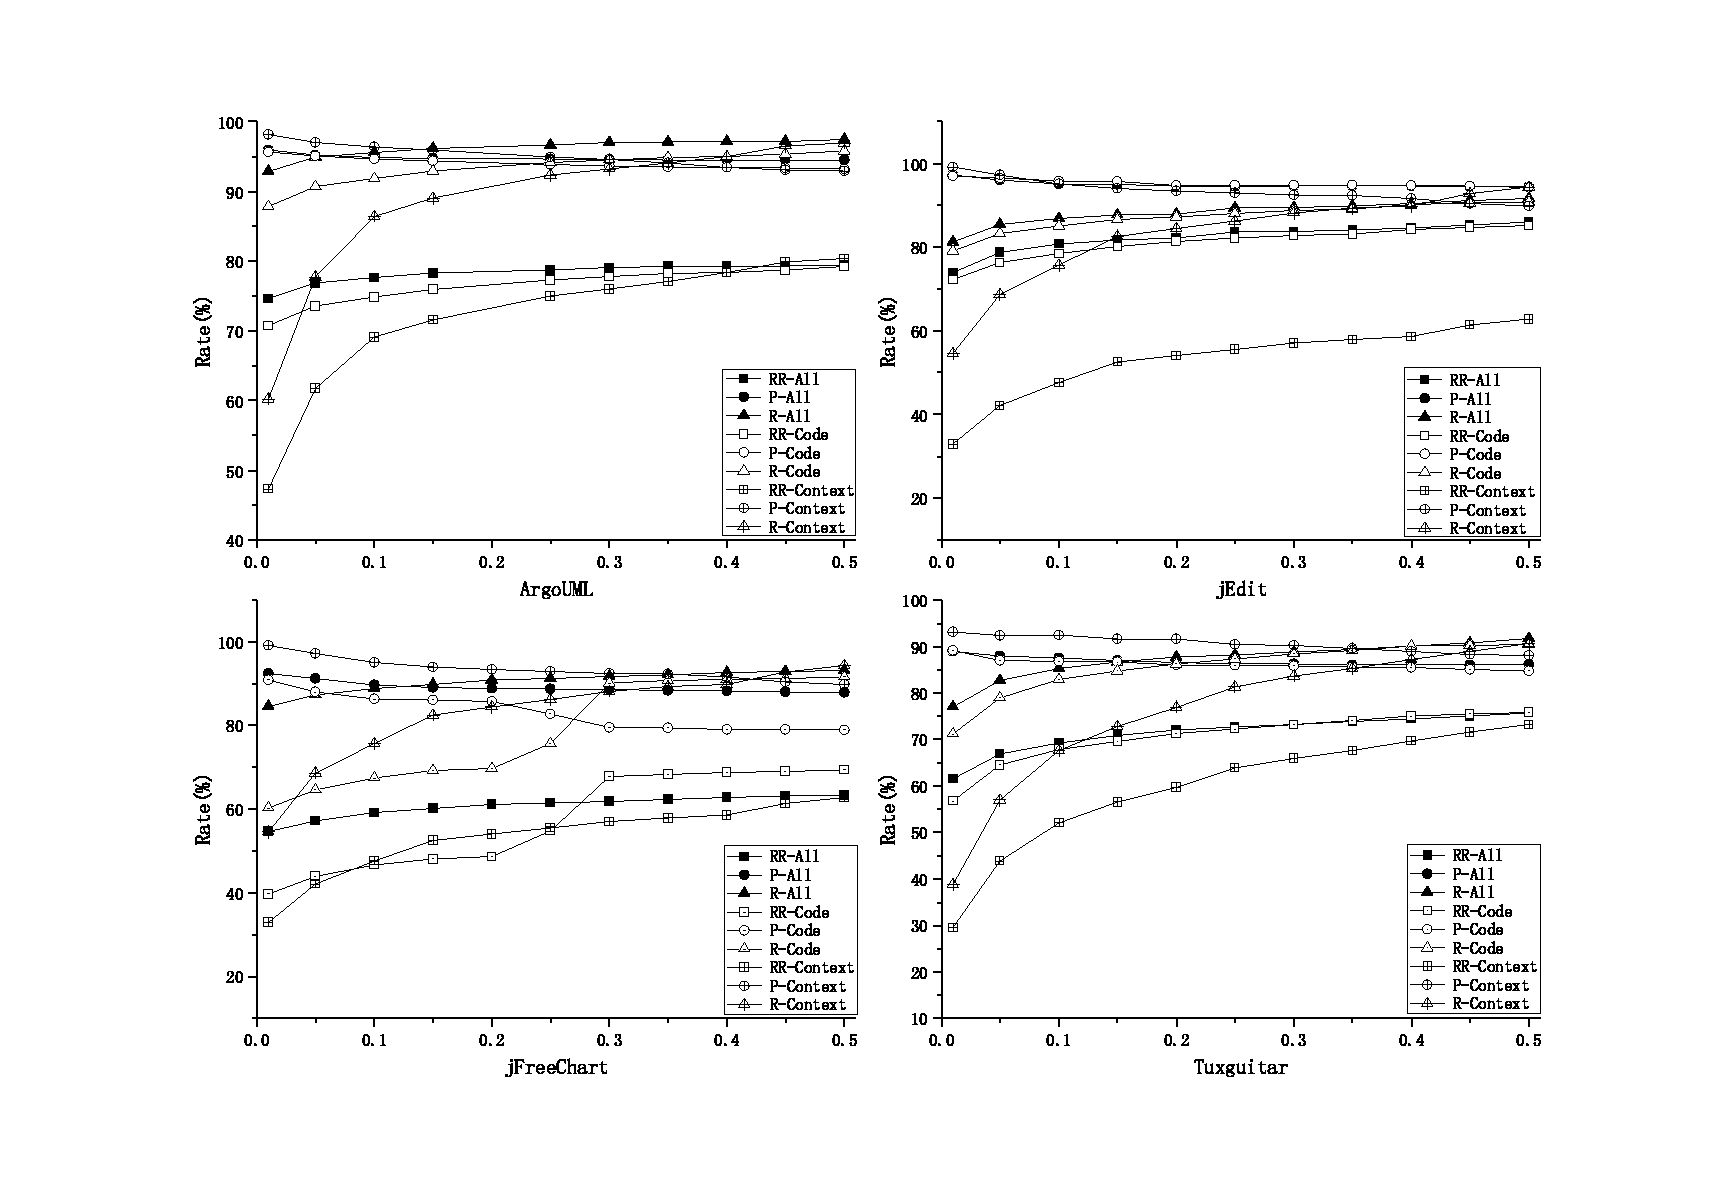
\includegraphics[width = 1.0\textwidth]{bayesgraph/creatingsetfree.pdf}
\bicaption[creatingsetfree]{}{属性组维护自由实验效果}
{Fig.$\!$}{The effectiveness for attribute set of clone consistency free}
\vspace{-1em}
\end{figure}

由图~\ref{creatingsetfree}~中可以看出,代码属性实验的预测效果依然较好,但和全属性实验对比发现代码属性实验的召回率下降,精确率除jEdit中少数几个之外也全部下降,因此本文提取的代码属性对预测作用具有积极意义。在上下文属性实验中,预测结果除jEdit系统外精确率提高,但是系统的召回率却大大降低。因此,下上下文属性对系统的精确率影响较大,而代码属性对系统的召回率影响较大,同时两者对于预测都起到了积极的作用。

因此,本章建议在进行预测时,保留所有的属性进行预测。因为某些属性可能对其它尚未验证的系统具有积极的作用。

%%%%实验结果如表~\ref{copysetfree}~所示,其中左侧为代码属性,右侧为上下文属性。由表~\ref{copysetfree}~和表~\ref{copyallfree}~中可以看出,代码属性实验的预测效果依然较好,但和全属性实验对比发现代码属性实验的召回率下降,精确率除jEdit中少数几个之外也全部下降,因此本文提取的代码属性对预测作用具有积极意义。在上下文属性实验中,预测结果除jEdit系统外精确率提高,但是系统的召回率却大大降低。因此,下上下文属性对系统的精确率影响较大,而代码属性对系统的召回率影响较大,同时两者对于预测都起到了积极的作用。
%%%%
%%%%因此,本章建议在进行预测时,保留所有的属性进行预测。因为某些属性可能对其它尚未验证的系统具有积极的意义。
%%%%
%%%%\begin{table}[htbp]
%%%%\bicaption[copysetfree]{}{属性组维护自由实验效果}
%%%%{Table$\!$}{The effectiveness for attribute set of clone consistency free}
%%%%\vspace{0.5em}
%%%%\centering
%%%%\wuhao
%%%%\begin{tabular}{cccccccc}
%%%%\toprule[1.5pt]
%%%%\multirow{2}{*}{实验系统}&\multirow{2}{*}{阈值}&\multicolumn{3}{c}{代码属性(\%)}&\multicolumn{3}{c}{上下文属性(\%)}\\
%%%%\cline{3-8}
%%%%&&推荐率&精确率&召回率&推荐率&精确率&召回率\\
%%%%\midrule[1pt]
%%%%\multirow{5}{*}{ArgoUML}
%%%%&0.01&	70.75&	95.64&	87.80&	47.31&	98.10&	60.22\\
%%%%&0.05&	73.53&	95.07&	90.71&	61.74&	96.99&	77.70\\
%%%%&0.1&	74.82&	94.60&	91.84&	69.22&	96.24&	86.44\\
%%%%&0.15&	75.93&	94.32&	92.93&	71.53&	95.90&	89.01\\
%%%%&0.2&	76.59&	94.02&	93.43&	73.59&	95.52&	91.22\\
%%%%\hline
%%%%\multirow{5}{*}{jEdit}
%%%%&0.01&	72.20&    96.94&	79.11&	32.95&	99.10&	54.60\\
%%%%&0.05&	76.30&	96.48&	83.21&	42.19&	97.25&	68.60\\
%%%%&0.1&	78.67&	95.78&	85.18&	47.74&	95.02&	75.86\\
%%%%&0.15&	80.09&	95.66&	86.61&	52.55&	93.95&	82.56\\
%%%%&0.2&	81.36&	94.76&	87.14&	54.10&	93.36&	84.45\\
%%%%\hline
%%%%\multirow{5}{*}{jFreeChart}
%%%%&0.01&	39.69&	90.94&	60.36&	32.95&	99.10&	54.60\\
%%%%&0.05&	43.94&	87.96&	64.63&	42.19&	97.25&	68.60\\
%%%%&0.1&	46.70&	86.32&	67.41&	47.74&	95.02&	75.86\\
%%%%&0.15&	48.07&	86.16&	69.25&	52.55&	93.95&	82.56\\
%%%%&0.2&	48.66&	85.71&	69.75&	54.10&	93.36&	84.45\\
%%%%\hline
%%%%\multirow{5}{*}{Tuxguitar}
%%%%&0.01&	56.75&	89.15&	71.16&	29.60&	93.14&	38.78\\
%%%%&0.05&	64.52&	86.98&	78.94&	43.88&	92.34&	56.99\\
%%%%&0.1&	67.88&	86.80&	82.87&	51.99&	92.46&	67.62\\
%%%%&0.15&	69.56&	86.62&	84.74&	56.54&	91.58&	72.83\\
%%%%&0.2&	71.24&	86.05&	86.22&	59.69&	91.56&	76.87\\
%%%%\bottomrule[1.5pt]
%%%%\end{tabular}
%%%%\end{table}

\BiSubsubsection{一致性维护需求实验}
{The Experiment for Meeting Clone Creating Consistency}

在本节中,对需要一致性维护的克隆创建实例进行评估。将关注需要一致性维护的克隆实例,由于其在演化过程中可能会引发一致性变化,因此需要警告程序开发人员谨慎的执行复制和粘贴操作,避免额外的维护代价。实验同样使用三个度量对方法进行评估:警告率、精确率和召回率。其中,警告率(Warning Rate)指所警告的需要一致性维护的克隆创建实例,即预测为需要一致性维护的实例与系统中全部实例的比值。

%%%\begin{itemize}
%%%\item	
%%%警告率(Warning Rate):
%%%指所警告的需要一致性维护的克隆创建实例,即预测为需要一致性维护的实例与系统中全部实例的比值。这些克隆实例可能会引发一致性变化和额外维护代价。
%%%\item	
%%%精确率(Precision):
%%%指警告为需要一致性维护的克隆创建实例的精确率,即在所预测的需要一致性维护的实例中,正确预测的实例与全部警告实例的比值。
%%%\item	
%%%召回率(Recall):指所警告的需要一致性维护的克隆创建实例的召回率,即预测为需要一致性维护的实例与系统中的需要一致性维护实例的比值。
%%%\end{itemize}

(1)全属性实验结果

全属性实验同样使用全部属性在四个实验系统上进行评估,实验结果如图~\ref{creatingallmeeting}所示。

\begin{figure}[h]
\centering
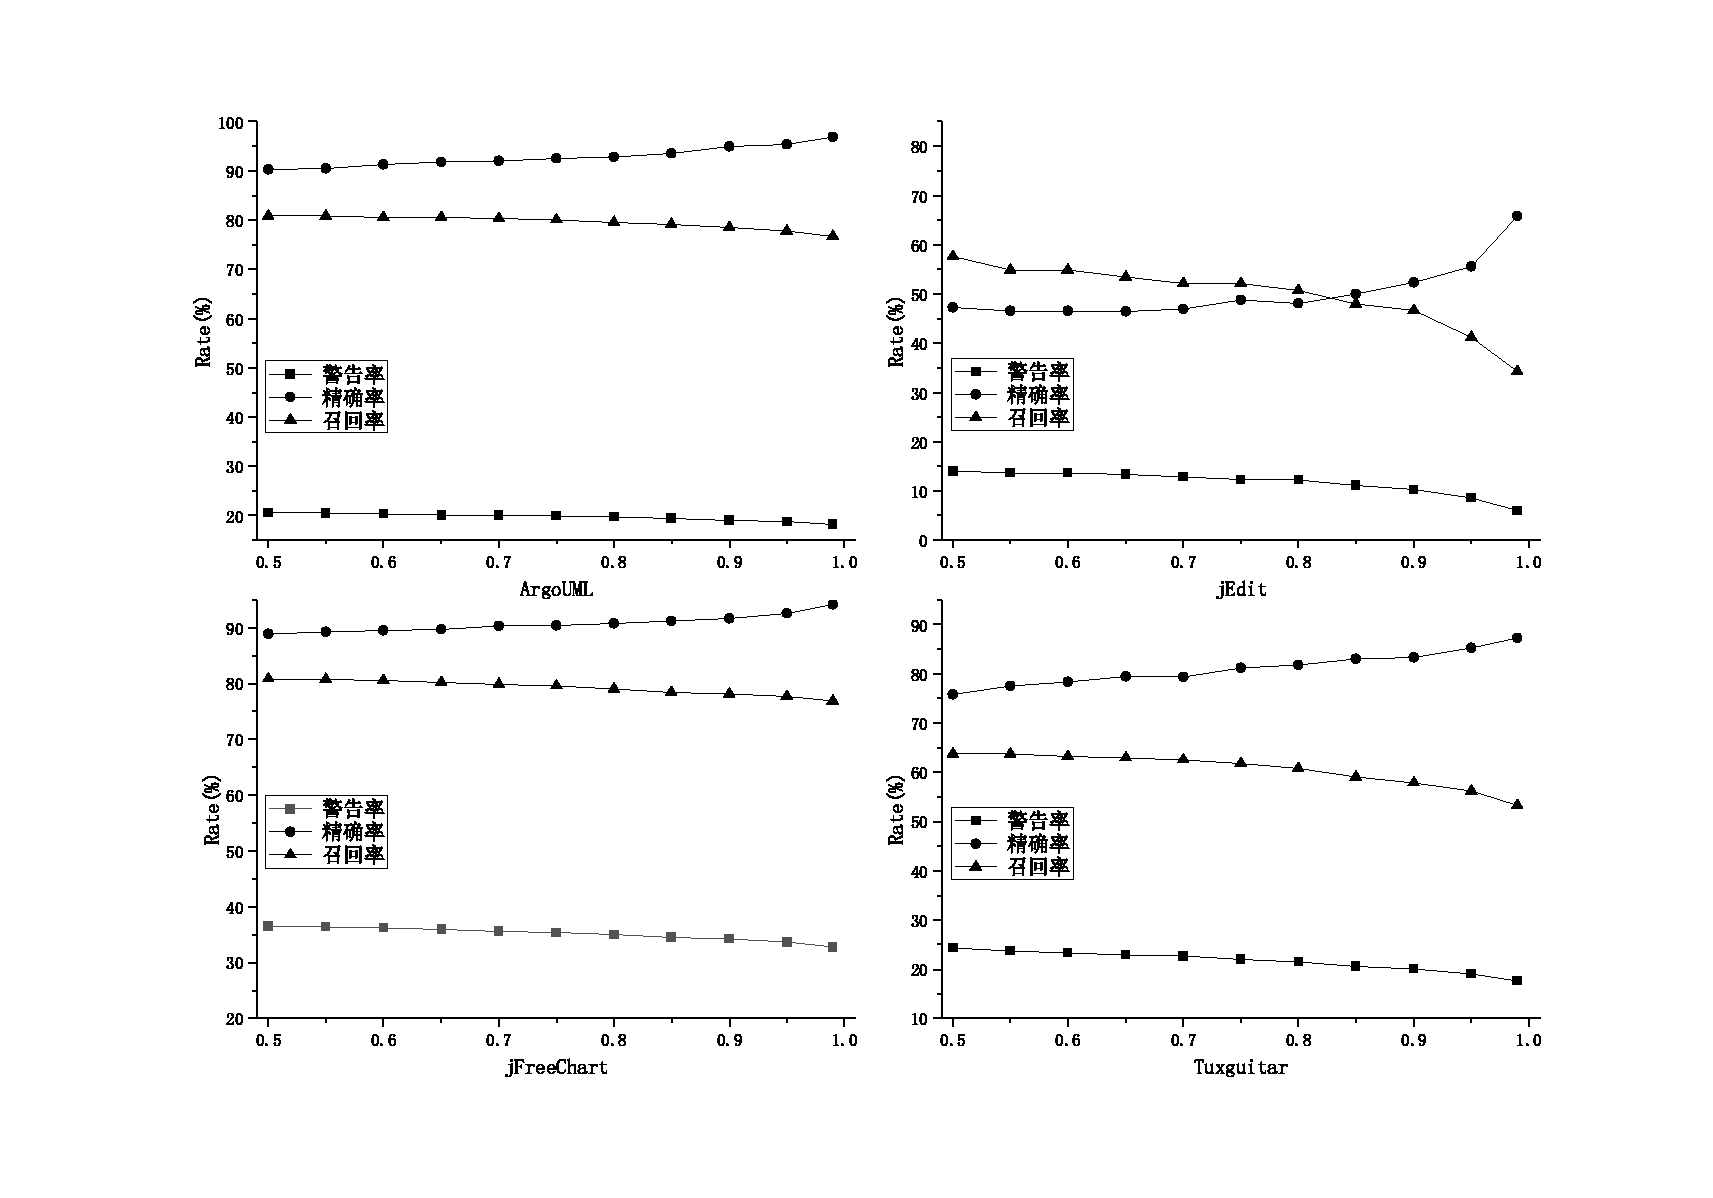
\includegraphics[width = 1.0\textwidth]{bayesgraph/creatingallmeeting.pdf}
\bicaption[creatingallmeeting]{}{全属性组需要维护的全属性实验效果}
{Fig.$\!$}{The effectiveness for all attributes of clone consistency}
\vspace{-1em}
\end{figure}

由图中可以看出,系统ArgoUML和jFreeChart在不同阈值下取得了可以不错的效果:精确率介于75.79\%-96.87\%之间,召回率介于76.63\%-80.86\%之间。尽管TuxGuitar的预测效果没有另外两个系统的预测结果差,但是其精确率在75.79\%-87.30\%,召回率为53.27\%-63.68\%。然而,jEdit系统的预测效果不够理想,其准确度和召回率仅在50\%左右。分析其原因可能为jEdit中训练数据过少导致模型不完全,数据集仅有73复制粘贴实例,仍需要进一步的研究确定。尽管如此,jEdit的预测结果的准确度依然高于其系统自身的一致性维护需求的比例(11.53\%)。因此,在jEdit系统上依然提高了预测的精度,也是有效的。最后,对于四个实验系统,本文所构建的模型均具有有十分合理的警告率,警告率十分接近于满足一致性维护需求的克隆变化实例的比例(如表~\ref {copysta}~中所示)。

虽然阈值的变化可以影响预测的精确率和召回率,但影响并不是十分的剧烈,其中除jEdit对精确率的影响要大于对召回率的影响。尽管如此,在不同的阈值下,本文构建模型的精确率依然达到了较高的水平。因此开发人员可以非常自信地依赖于本文模型的预测结果。然而,本文方法的召回率没有达到准确两率的效果,但仍需进一步增强预测模型的召回能力,这需要进一步的深入研究。


%%%%全属性实验同样使用全部属性在四个实验系统上进行评估,实验结果如表~\ref{copyallmeeting}所示。由表中可以看出,除jEdit外其余系统在不同阈值下取得了可以不错的效果:精确率介于75.79\%-94.94\%之间,召回率介于57.87\%-80.86\%之间。jEdit的预测效果不够理想,其准确度和召回率仅在50\%左右。分析其原因可能为jEdit中训练数据过少导致模型不完全,数据集仅有73复制粘贴实例,仍需要进一步的研究确定。尽管如此,jEdit的预测结果的准确度依然高于其系统自身的一致性维护需求的比例(11.53\%)。因此,在jEdit系统上依然提高了预测的精度,也是有效的。最后,对于四个实验系统,本文所构建的模型均具有有十分合理的警告率,警告率十分接近于满足一致性维护需求的克隆变化实例的比例(如表~\ref {copysta}~中所示)。
%%%%
%%%%虽然阈值的变化可以影响预测的精确率和召回率,但影响并不是十分的剧烈,其中除jEdit对精确率的影响要大于对召回率的影响。尽管如此,在不同的阈值下,本文构建模型的精确率依然达到了较高的水平。因此开发人员可以非常自信地依赖于本文模型的预测结果。然而,本文方法的召回率没有达到准确两率的效果,但仍需进一步增强预测模型的召回能力,这需要进一步的深入研究。
%%%%
%%%%\begin{table}[htbp]
%%%%\bicaption[copyallmeeting]{}{需要维护的全属性实验效果}
%%%%{Table$\!$}{The effectiveness for all attributes of clone consistency}
%%%%\vspace{0.5em}
%%%%\centering
%%%%\wuhao
%%%%\begin{tabular}{ccccc}
%%%%\toprule[1.5pt]
%%%%{实验系统}&{阈值}&{警告率(\%)}&{精确率(\%)}&{召回率(\%)}\\
%%%%\midrule[1pt]
%%%%\multirow{5}{*}{ArgoUML}
%%%%&0.9&	18.95&	94.94&	78.46\\
%%%%&0.8&	19.64&	92.84&	79.50\\
%%%%&0.7&	20.03&	91.93&	80.29\\
%%%%&0.6&	20.24&	91.27&	80.55\\
%%%%&0.5&	20.54&	90.23&	80.81\\
%%%%\hline
%%%%\multirow{5}{*}{jEdit}
%%%%&0.9&	10.27&	52.31&	46.58\\
%%%%&0.8&	12.16&	48.05&	50.68\\
%%%%&0.7&	12.80&	46.91&	52.05\\
%%%%&0.6&	13.59&	46.51&	54.79\\
%%%%&0.5&	14.06&	47.19&	57.53\\
%%%%\hline
%%%%\multirow{5}{*}{jFreeChart}
%%%%&0.9&	34.25&	91.67&	78.12\\
%%%%&0.8&	35.03&	90.75&	79.08\\
%%%%&0.7&	35.56&	90.31&	79.90\\
%%%%&0.6&	36.19&	89.49&	80.56\\
%%%%&0.5&	36.57&	88.87&	80.86\\
%%%%\hline
%%%%\multirow{5}{*}{Tuxguitar}
%%%%&0.9&	20.08&	83.28&	57.87\\
%%%%&0.8&	21.48&	81.76&	60.77\\
%%%%&0.7&	22.74&	79.38&	62.47\\
%%%%&0.6&	23.30&	78.38&	63.20\\
%%%%&0.5&	24.28&	75.79&	63.68\\
%%%%\bottomrule[1.5pt]
%%%%\end{tabular}
%%%%\end{table}

(2)属性组实验结果

类似的,对于一致性维护需求实例,表~\ref{creatingsetmeeting}~给出了属性组实验结果。其中,使用“WR”表示警告率,“P”表示精确率,“R”表示召回率。并同时使用不同的后缀表示不同属性组的实验结果,其中“All”为全属性组实验结果,“Code”表示仅使用代码属性的实验结果,“Context”表示上下文属性的实验结果。

\begin{figure}[h]
\centering
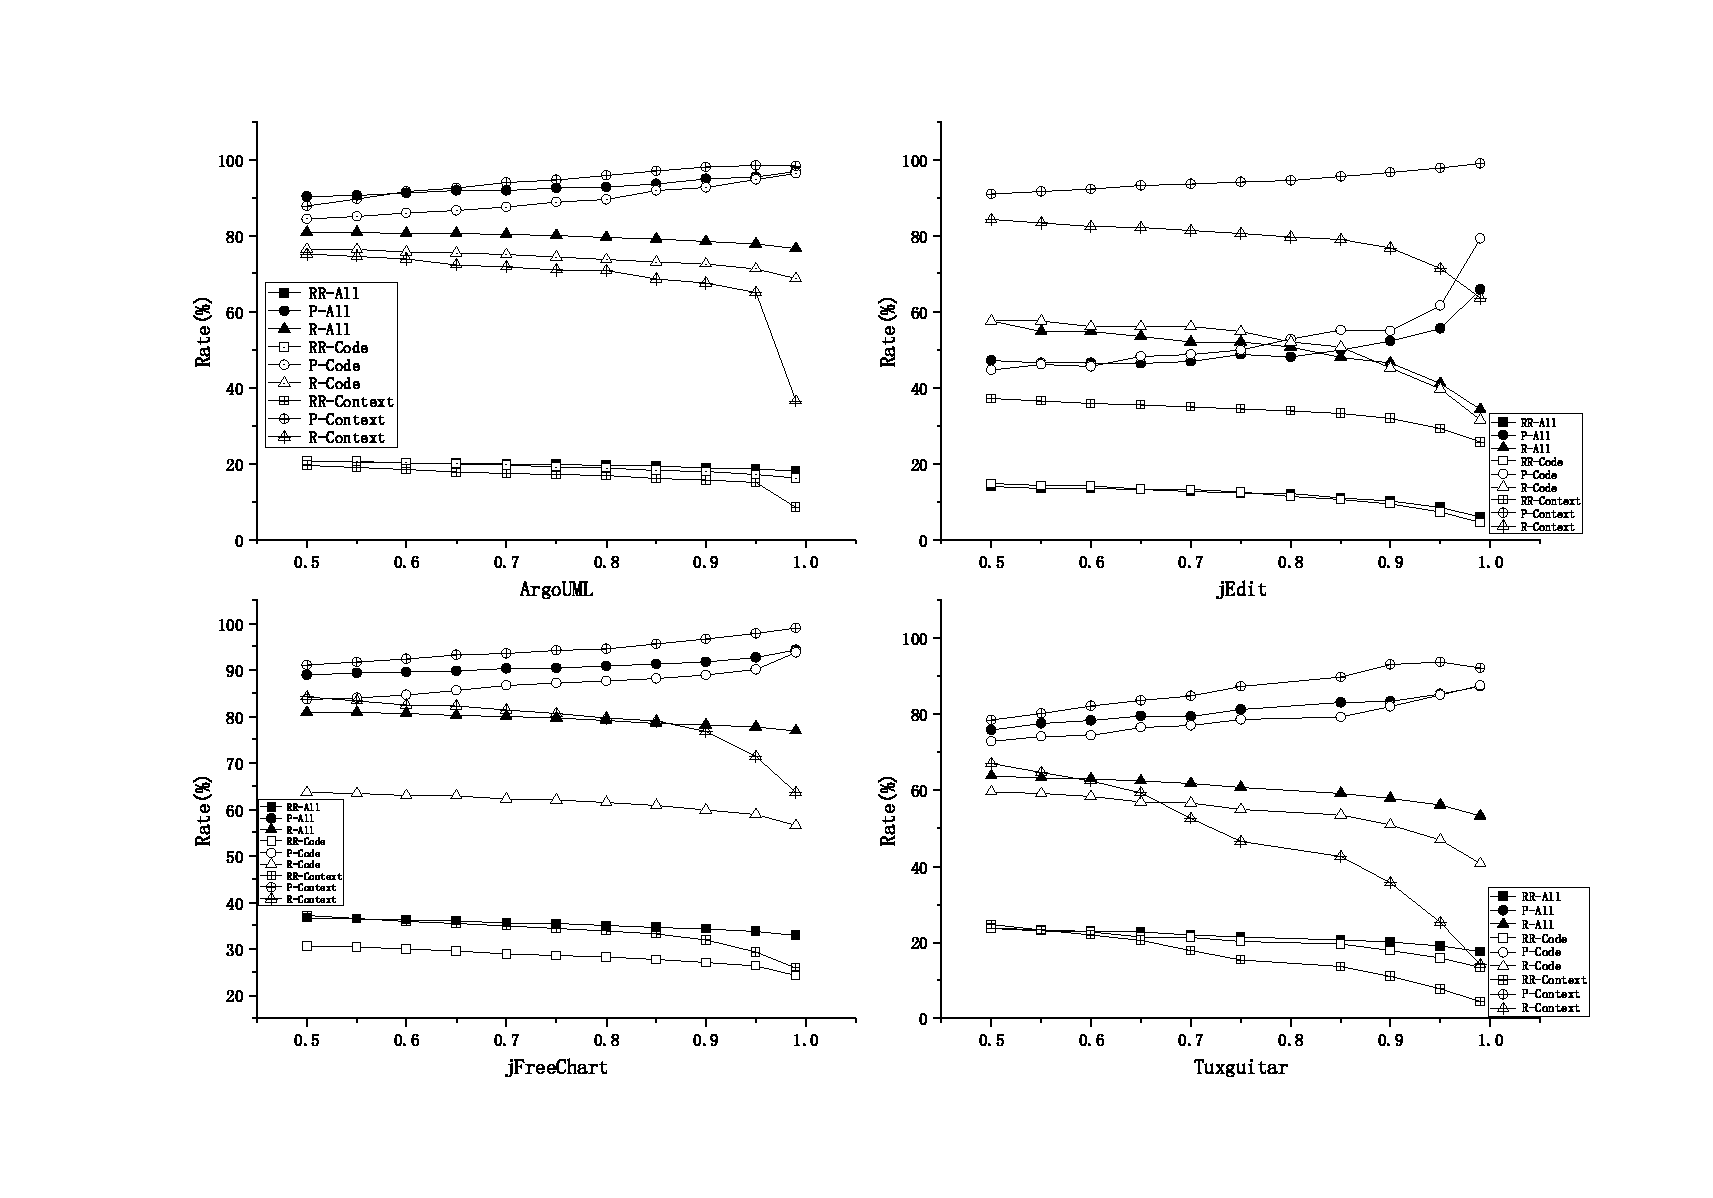
\includegraphics[width = 1.0\textwidth]{bayesgraph/creatingsetmeeting.pdf}
\bicaption[creatingsetmeeting]{}{需要维护的属性组实验效果}
{Fig.$\!$}{The effectiveness for attribute set of clone consistency}
\vspace{-1em}
\end{figure}

由图中可以看出,代码属性的实验结果明显不如全属性组实验,但仍在可接受的范围之内,说明代码属性对预测有积极的影响。上下文属性实验中,当仅仅使用上下文属性时部分系统的实验效果要优于全属性组实验,而部分系统的结果不如全属性组实验。因此,上下文属性对不同的系统所起到的作用并非一样的。上下文属性和代码属性都具有积极地意义,而上下文属性的影响更大。


%%%%%类似的,对于一致性维护需求实例,表~\ref{copysetmeeting}~给出了属性组实验结果。由表中可以看出,代码属性的实验结果明显不如全属性组实验,但仍在可接受的范围之内,说明代码属性对预测有积极的影响。上下文属性实验中,当仅仅使用上下文属性时部分系统的实验效果要优于全属性组实验,而部分系统的结果不如全属性组实验。因此,上下文属性对不同的系统所起到的作用并非一样的。上下文属性和代码属性都具有积极地意义,而上下文属性的影响更大。
%%%%%
%%%%%\begin{table}[htbp]
%%%%%\bicaption[copysetmeeting]{}{需要维护的属性组实验效果}
%%%%%{Table$\!$}{The effectiveness for attribute set of clone consistency}
%%%%%\vspace{0.5em}\centering\wuhao
%%%%%\begin{tabular}{cccccccc}
%%%%%\toprule[1.5pt]
%%%%%\multirow{2}{*}{系统}&\multirow{2}{*}{阈值}&\multicolumn{3}{c}{ 代码属性(\%)}&\multicolumn{3}{c}{上下文属性(\%)}\\
%%%%%\cline{3-8}
%%%%%&&{警告率}&{精确率}&{召回率}&{警告率}&{精确率}&{召回率}\\
%%%%%\midrule[1pt]
%%%%%\multirow{5}{*}{ArgoUML}
%%%%%&0.9&	17.96&	92.67&	72.58&	15.78&	98.10&	67.49\\
%%%%%&0.8&	18.89&	89.54&	73.76&	16.98&	95.77&	70.89\\
%%%%%&0.7&	19.67&	87.52&	75.07&	17.51&	94.02&	71.80\\
%%%%%&0.6&	20.21&	85.93&	75.72&	18.50&	91.59&	73.89\\
%%%%%&0.5&	20.78&	84.44&	76.50&	19.64&	87.80&	75.20\\
%%%%%\hline
%%%%%\multirow{5}{*}{jEdit}
%%%%%&0.9&	9.48&	55.00&	45.21&	31.91&	96.65&	76.72\\
%%%%%&0.8&	11.37&	52.78&	52.05&	33.87&	94.47&	79.60\\
%%%%%&0.7&	13.27&	48.81&	56.16&	34.94&	93.54&	81.30\\
%%%%%&0.6&	14.22&	45.56&	56.16&	35.89&	92.30&	82.41\\
%%%%%&0.5&	14.85&	44.68&	57.53&	37.20&	90.97&	84.18\\
%%%%%\hline
%%%%%\multirow{5}{*}{jFreeChart}
%%%%%&0.9&	27.04&	88.90&	59.79&	31.91&	96.65&	76.72\\
%%%%%&0.8&	28.19&	87.57&	61.42&	33.87&	94.47&	79.60\\
%%%%%&0.7&	28.85&	86.61&	62.16&	34.94&	93.54&	81.30\\
%%%%%&0.6&	29.92&	84.61&	62.97&	35.89&	92.30&	82.41\\
%%%%%&0.5&	30.57&	83.58&	63.56&	37.20&	90.97&	84.18\\
%%%%%\hline
%%%%%\multirow{5}{*}{Tuxguitar}
%%%%%&0.9&	17.91&	82.03&	50.85&	11.06&	93.04&	35.59\\
%%%%%&0.8&	20.22&	78.55&	54.96&	15.40&	87.27&	46.49\\
%%%%%&0.7&	21.48&	76.55&	56.90&	20.50&	83.62&	59.32\\
%%%%%&0.6&	23.02&	74.16&	59.08&	23.30&	80.18&	64.65\\
%%%%%&0.5&	24.14&	71.88&	60.05&	26.94&	74.81&	69.73\\
%%%%%\bottomrule[1.5pt]
%%%%%\end{tabular}
%%%%%\end{table}

\BiSubsection{与其它方法的对比}
{Comparing with Wang’s Method}

Wang\cite{wang2014predicting}等人也使用贝叶斯网络对克隆代码创建时的一致性维护需求进行了研究。其在四个实验系统上进行了实验,其中两个实验系统是微软内部的系统,另外两个系统为开源系统jFreeChart和Tuxguitar。因此,本节将本章的实验结果与Wang的方法进行对比,从而验证本章所提出方法的有效性。方法对比的实验结果如表~\ref{comparecopysta}~和表~\ref{comparecopyprediction}~所示。

\begin{table}[htbp]
\bicaption[comparecopysta]{}{实验系统的克隆创建实例信息统计对比}
{Table$\!$}{The comparing statistics for clone creating instances in four projects}
\vspace{0.5em}
\centering
\wuhao
\begin{tabular}{cccc}
\toprule[1.5pt]
~\multirow{2}{*}{实验系统}& \multicolumn{2}{c}{克隆变化实例的数量(比例)} & \multirow{2}{*}{总数}\\ 
 \cline{2-3}
~&{不需要维护} &{需要维护} & ~\\
\midrule[1pt]
jFreeChart(本章)&	2013(59.8\%)&	1353(40.2\%)&	3366\\
jFreeChart(Wang)&1059(92.2\%)&	89(7.8\%)&	1148\\
Tuxguitar(本章)&	1016(71.1\%)&	413(28.9\%)&	1429\\
Tuxguitar(Wang)&384(86.5\%)&	60(13.5\%)&	444\\
\bottomrule[1.5pt]
\end{tabular}
\end{table}

\begin{table}[htbp]
\bicaption[comparecopyprediction]{}{实验系统的克隆创建实例信息统计对比}
{Table$\!$}{The comparing effectiveness for clone creating instances in two projects}
\vspace{0.5em}
\centering
\wuhao
\begin{tabular}{ccc}
\toprule[1.5pt]
{实验系统}&{平均精确率} &{平均召回率}\\ 
\midrule[1pt]
jFreeChart(本章)&	88.3\%& 88.2\%\\
jFreeChart(Wang)&58.3\%&	63\%\\
Tuxguitar(本章)&	83.1\%&	83.6\%\\
Tuxguitar(Wang)&61.5\%&	60.1\%\\
\bottomrule[1.5pt]
\end{tabular}
\end{table}

表~\ref{comparecopysta}~是所收集到的克隆创建实例信息对比。由表中可以看出,本章所收集的克隆创建实例数量要多于Wang所收集的。
表~\ref{comparecopyprediction}~是本章方法与Wang的方法的预测效果对比。表中使用平均精确度(Average Precision)和平均召回率(Average Recall)评估预测效果,即加权平均需要和不需要一致性维护的预测结果。
由表中可以看出,本章所提出的方法优于Wang所提出的方法。


\BiSubsection{讨论}
{Discussion}

本节从不同的角度评估了本章所提出的克隆代码创建的一致性维护需求预测,同时对不需要和需要一致性维护需求的克隆创建实例进行了预测,并从不同的角度评估了不同的机器学习方法的预测能力。

在机器学习方法对比中,在克隆代码创建时,五种机器学习方法都可应用于克隆代码的一致性维护需求预测中,并具有相似的预测能力,预测结果具有较高的精确率、召回率和F值。更重要的是,不同机器学习模型的预测能力仅具有较小的差异,但SVM方法拥有相对最佳的预测效果。因此,建议优先推荐使用SVM方法,预测克隆代码创建的一致性维护需求。与此同时,所提取的属性组作为一个整体在不同机器学习方法的预测中,同样起到了积极的作用。因此,建议软件开发人员在预测时保留所有的属性组进行创建时一致性预测。

在使用贝叶斯网络方法的预测中,全属性实验结果表明:本章所构建的模型在一致性维护需求和一致性维护自由的实验上,均具有高效地预测能力。同时,本文所提取的代码属性和上下文属性对克隆创建实例的一致性维护需求的预测起到了积极的作用。但在不同系统中,所产生的影响程度不一致。因此,建议维护人员使用全属性组进行克隆创建实例的一致性维护需求预测,从而将其适用到其它未验证的系统中,使之达到最佳的预测效果。此外,与Wang提出的方法进行了对比,结果表明本章所提出的方法具有更好的预测能力。

\BiSection{本章小结}
{Summary of this Chapter}

通过复制和粘贴操作复用既有代码可以向系统中引入新创建的克隆代码,然而在其演化过程中可能会发生一致性变化,从而导致额外的维护代价。为帮助软件开发人员避免克隆代码的额外维护代价,本章提出了一个克隆代码创建一致性维护需求预测方法。可在克隆代码创建时(复制和粘贴时),预测新创建的克隆代码的一致性维护需求,根据预测结果决定是否执行该复制粘贴操作。构建了软件系统的克隆家系,并通过识别克隆家系的根节点收集克隆创建实例(复制和粘贴操作)。使用不同的属性组表示克隆创建实例,使用代码属性表示被复制克隆代码,使用上下文属性表示被粘贴的克隆代码。在四个开源软件系统上进行实验,验证所构建模型的预测能力。实验结果表明本章方法可以以较高的精确率和召回率高效地预测克隆代码的一致性维护需求。此外,所提取的两组属性组在预测中均起到了积极的作用,但是对精确率和召回率有不同的影响。

%本文的主要贡献如下:
%(1)本文定义了新的克隆代码一致性变,并根据其定义了克隆代码的一致性维护需求,可以更为准确的标识克隆代码的一致性维护代价;
%(2)本文使用并扩展代码属性和上下文属性两组属性组,实验结果表明所使用的属性在克隆一致性维护需求的预测中起到了积极的作用;
%(3)本文预测克隆代码的一致性维护需求,不仅在贝叶斯网络分类器上进行了实验评估,还在一般分类器上进行了实验验证,实验结果表明本文方法具有一般性,可以适用于一般的机器学习方法。